%%%%%%%%%%%%%%%%%%%%%%%%%%%%%%%%%%%%%%%%%%%%%%%%%%
%
%  This chapter is now in good condition
%
%%%%%%%%%%%%%%%%%%%%%%%%%%%%%%%%%%%%%%%%%%%%%%%%%%

%
% change log:
% revised at 12th, July 2009
% now seems to be satisfied with all the contents
% list the contents here:
% 1  introduction of the density VS. wave functions
% 2  HK theorem
% 3  make HK theorem more precise, Levy research; introduce the F_nk[n]
% 4  introduce the concept of non-interacting system, so that
%    to physically express the total energy 
% 5  use a more strict way(adiabatic connection) to get the total energy
%    again, and get the expression for exc;
% 6  based on the total energy expression, we get Kohn-Sham equation;
% 7  extend to spin-polarized case;
% 8  what does Ts[rho] physically mean? Give some interpretation.



\chapter{Introduction to Density Functional Theory}
%%%%%%%%%%%%%%%%%%%%%%%%%%%%%%%%%%%%%%%%%%%%%%%%%%%%%%%%%%%%%%%%%%%%%%%%%%%%%%
\section{Another way to understand Schrodinger equation}
%
% reveals that the Hamiltonian operator only contains the information
% of number of electrons and the position of nucleus(also its total
% number).  thus we can find a way to solve another equation, in which
% the operators also give the same information.  that's some original
% suspect for the DFT
%
%
On the base of Born-Oppenheimer approximation, the electron Hamilton
is separated from the total schrodinger equation. The whole analysis
of the quantum chemistry, is concentrated on the electron wave
function, which is solved from the electron schrodinger equation:

\begin{equation}\label{DFTIeq:2}
  \left\{\sum_{i=1}^{n}(\frac{-1}{2}\times\nabla_{i}^2)
    +\sum_{i=1}^{n}\sum_{\alpha=1}^{N}
    (\frac{-1}{r_{i\alpha}})+\sum\sum_{i<j}(\frac{1}{r_{ij}})
  \right\}\,\Psi=E\Psi
\end{equation}

What kind of information is included in the $\hat{H}$? This is some
very interesting problem, and through answering this problem, we may
be get some general and crude aspects about how to understand the
Schrodinger equation in another way.

For any given $\Psi$, The kinetic operator is irrelevant so kinetic
operator just reflects the information of number of electrons
through the sum symbol in the (\ref{DFTIeq:2}). The nuclear-electron
operator tells that the specific orientation of the nucleus as well
as its total number. At last the electron repulsion operator is only
including the information related to the number of electrons; which
is roughly the same to the kinetic operator.

So far we can summarize the crude estimation we made for the
information included in the $\hat{H}$\,:
\begin{itemize}
\item the location and the number of nuclear
\item the number of electrons
\end{itemize}

Here the results implies that if the same information can be produced
by another operator, which may be similar to the $\hat{H}$\,; perhaps
we can get the same answer as solving the schrodinger equation.

Furthermore, the discussion related to the density matrices offers
us another point of view to understand the Schrodinger equation. The
Schrodinger equation can be expressed by the density matrices as:
\begin{eqnarray}\label{DFTIeq:5}
  E=tr(\hat{H}\hat{\gamma})=\int\hat{H_{1}}
  \Big(\hat{\gamma_{1}}(x_{1}^{'}\,,x_{1})\Big)_{x_{1}^{'}=x_{1}}\,dx_{1}+
  \nonumber \\
  \int\hat{H_{2}}\Big(\hat{\gamma_{2}}
  (x_{1}^{'}\,,x_{2}^{'}\,,x_{1}\,,x_{2})\Big)_{x_{1}^{'}
    =x_{1}\,,x_{2}^{'}=x_{2}}\,dx_{1}dx_{2}
\end{eqnarray}

The $\hat{H_{1}}$ denotes the operator acting on the single
electron; $\hat{H_{2}}$ denotes the operator acting on the double
electrons. So here it's concluded that the information of the
$\hat{H}$ can be expressed by the fist order of density matrices and
the second order of density matrices. Therefore, the result
demonstrates a well known fact that in principle, the total wave
function with its complicated dependence on the N electron
coordinates, is not necessary to obtain the energy; the reduced
first order and second order density matrices are sufficient.

From the further result given by Davidson\cite{Davidson}, we are
instructed to know that for the $\rho_{1}(x_{1})$, it possess some
interesting characters:
\begin{eqnarray}\label{}
  \int\rho(\vec{r})\,d\vec{r}=N \\
  \lim_{\vec{r}_{iA}\rightarrow 0}\left
    [ {\frac{\partial}{\partial r}}+2Z_{A}\right ]\rho(\vec{r})=0
\end{eqnarray}

The second theorem says that while the electron approaches nearer to
the nuclear($\vec{r_{iA}}\rightarrow 0$), the differentiation of
$\rho(\vec{r})$ to the $\vec{r_{iA}}$ tends to be $-2Z_{A}\times
\rho(\vec{r})$.

So we can see that the information with respect to the nuclear and
electrons given by $\hat{H}$ also demonstrates in the $\rho(\vec{r})$,
just as what we have suspected. Therefore, we put forward a question
that whether the $\rho(\vec{r})$ can give the same information just as
the $\hat{H}$ ? That's some questions left for the future answer, and
by reckoning this hypothesis, we can start the DFT voyage.



%%%%%%%%%%%%%%%%%%%%%%%%%%%%%%%%%%%%%%%%%%%%%%%%%%%%%%%%%%%%%%%%%%%%%%%%%
\section{The Hohenberg-Kohn theorems}
%
% proof of existence of DFT theory prove that the rho can be used as
% variation principle
%
%

To people's surprise, the foundation of DFT theory is rather simple
and straightforward. Even though there had been existing Thomas-fermi
model for nearly 40 years, until 1965 none of the people had paid
little attention to the possibility to establish a new theory on the
base of $\rho(\vec{r})$; and such theory should be emphasized that
it's equivalent to the schrodinger equation\footnote{Here, the author
  is try to recommend some materials which is helpful to understand
  the DFT. The people with physical background may prefer the book by
  Gross\cite{Gross_DFT}, and the people with mathematical background
  may prefer the book by Eschrig
  H.\cite{Fundamentals_of_Density_Functional_Theory}. Furthermore, the
  chemists should refer to the book by the Parr and
  Weitao\cite{weitaoYang}, but compared with the Gross book, this book
  is a bit of general and not be precise conceptually. There are some
  other books and materials that the chemists can be
  refereed\cite{argaman-1998, capelle-2002, RevModPhys.61.689, Koch,
    DFT_Basics_New_Trends_and_Applications,
    Density_Functional_Theory_I, Density_Functional_Theory_III}
  etc. Here th author recommend the \cite{Koch} and
  \cite{DFT_Basics_New_Trends_and_Applications}, and we have found
  that the material from Professor Barth\cite{2004PhST..109....9V} is
  very enlightening.}.

So, it finally comes in 1965\cite{HK1}.

\subsection{The first theorem: proof of existence}
%
% the basic idea of the HK theorem all the operator in DFT is
% functional on density. some new understanding
%
Basically, the first theorem sets up an one to one mapping
relationship between the external potential of $v(r)$ and the ground
state electron density of $\rho(r)$. the first Hohenberg-Kohn theorem
states:
\begin{itemize}
\item The external potential $v(r)$ (within a constant) is the unique
  functional of $\rho(r)$; since that in turn the $v(r)$ fixes
  Hamiltonian, then we see that the full many particle ground state is
  a unique functional of electron density.
\end{itemize}

Now let's prove this theorem.

Suppose there's two $\hat{H}$ and $\hat{H^{'}}$\,, they represent two
different system by more than a constant. So the above explanation
means: $\hat{H}\neq C\times\hat{H^{'}}$. And both of the system here
have the same $\rho$ to describe it's ground state.  Because
$\hat{H}\neq C\times\hat{H^{'}}$, the true wave functions of $\psi$
for $\hat{H}$; and $\psi^{'}$ for $\hat{H^{'}}$ are totally different.


To the $\hat{H}$, we take the $\psi^{'}$ as a trial function and by
the virtue of variational principle; we have:
\begin{eqnarray}\label{DFTIeq:6}
  % \nonumber to remove numbering (before each equation)
  E_{0} &=& \langle\psi|\hat{H}|\psi\rangle   \nonumber  \\
  E_{0} &<& \langle\psi^{'}|\hat{H}|\psi^{'}\rangle =
  \langle\psi^{'}|\hat{H^{'}}|\psi^{'}\rangle +
  \langle\psi^{'}|\hat{H}-\hat{H^{'}}|\psi^{'}\rangle
\end{eqnarray}
which yields:
\begin{equation}\label{DFTIeq:3}
  E_{0} < E_{0}^{'} + \int\rho(r)(v(r)-v(r^{'}))\,dr
\end{equation}

Here the $\hat{H}-\hat{H^{'}}$ leaves only for the terms related to
the nuclear, since the other terms (kinetic and repulsion) are the
same.

By transposing the position of $\psi$ with $\hat{H}$, and $\psi^{'}$
with $\hat{H}^{'}$; we can get the similar result:
\begin{equation}\label{DFTIeq:4}
  E_{0}^{'} < E_{0} + \int\rho(r)(v(r^{'})-v(r))\,dr
\end{equation}

If we add the (\ref{DFTIeq:3}) and the (\ref{DFTIeq:4}) together,
simply we can get :$ E_{0}+E_{0}^{'} < E_{0}+E_{0}^{'} $; which is
obviously contradictive. So from here we can say that the
Hohenberg-Kohn theorem is true.

In this proof some kind of strong restriction is introduced; which
denotes that the ground state of $\hat{H}$ should be
non-degenerated. Actually if the ground states are degenerated, that
implies for the ground state we have different $\psi$ corresponding to
it, hence we may have different $\rho$ corresponding to the $v(r)$;
then the one to one mapping between the external potential and the
electron density has to be broken. That's the situation the HK theorem
can not deal with.

However, when the DFT theory proceeds to the next stage of Levy
constraint search, it's clear demonstrated that this restriction on
DFT foundation is eliminated.

The HK theorem shed new lights to the understanding on the old
quantum mechanics, which is totally based on the wave functions and
the operators. In the traditional quantum mechanics, the wave
function contains all the system information and we use operator to
determine it and extract the information from the wave functions.
Now similarly we has proved that the status of wave function can be
replaced the density, and the operator on the wave function can be
revised to be the functionals on the density. In the previous
chapter, in the discussion of the density matrices; we already has
seen such idea that the description within quantum chemistry can be
proceed only with density matrices. Now from the HK theorem it has
shown that the density is enough.
\begin{align}\label{}
  \text{density} &\Leftrightarrow \text{wave function} \nonumber \\
  \text{functional} &\Leftrightarrow \text{operator}
\end{align}


%%%%%%%%%%%%%%%%%%%%%%%%%%%%%%%%%%%%%%%%%%%%%%%%%%%%%%%%%%%%%%%%%%%%%%%%%%%
\subsection{The second theorem: variational principle}

Upon the first theorem, the proof of second theorem\cite{HK1} is quiet
straightforward.

Since the theorem 1 says that $\hat{H}$ has only one $\rho(r)$
describing its ground state, so that the $\rho(r)$ must be the one
which makes the lowest energy state, and other trial $\rho(\tilde{r})$
makes higher energy state; thus the $\rho(r)$ corresponds to the
ground state must achieve the minimum of the energy, that's what
requires by the variation principle:
\begin{equation}\label{}
  E_{0}< E(\rho(\tilde{r}))
\end{equation}
in which the $\rho(\tilde{r})$ is the different $\rho$ with respect to
the fixed $\hat{H}$. Upon this equation, now it's facilitated to make
variational research on $\rho$.


%%%%%%%%%%%%%%%%%%%%%%%%%%%%%%%%%%%%%%%%%%%%%%%%%%%%%%%%%%%%%%%%%%%%%%%%%%%
\section{The Levy constraint search approach}\label{DFTI:1}
%
% 1 what's the problems behind the HK theorem?  2 how to conquer them?
%
%
%
%
%
\subsection{Problems in The HK Theorem}

There's some mystery still around the HK theorem, not only the the
condition of non-degenerate states. A density is called
\emph{v-representable} if this density associated with the
antisymmetric ground state wave function of a Hamiltonian with some
external potential $v(r)$. So on the base of the definition, HK
theorem can be expressed as the one to one mapping between
v-representable density, the Hamiltonian of $\hat{H}$ and the ground
state wave function of $\psi$.
\begin{equation}\label{DFTIeq:1}
  \psi \Leftrightarrow \hat{H} \Leftrightarrow \rho(r)
\end{equation}


There exist some density which is not \emph{v-representable} indeed,
such example has been demonstrated in the book by Parr and
Weitao\cite{weitaoYang}. So conceptually the variational search can
not include the trial density which is not \emph{v-representable}.  So
it's a big problem.

However, by a simple demonstration, Levy\cite{levy1, levy2} has proved
that there indeed a one to one mapping between density and the
external potential of $v(r)$, as long as the density is
\emph{N-representable}; that is to say; the density can be obtained
from some antisymmetric wave functions. This condition is weaker than
the \emph{v-representable} condition, and the proof guarantees the
feasibility of variational search.

In Parr and Weitao 's book, they showed that a density $\rho(r)$ is
\emph{N-representable} if:
\begin{eqnarray}
  % \nonumber to remove numbering (before each equation)
  \rho(r) &\geq& 0 \nonumber \\
  \int \rho(r) dr &=&  N \nonumber \\
  \int | \nabla \rho(r)^{1/2} |^{2} dr &<& \infty
\end{eqnarray}
Such condition can be satisfied by the N orthogonal orbitals ,
therefore, the Levy theorem has lifted the final stone of the
foundation of DFT.

%%%%%%%%%%%%%%%%%%%%%%%%%%%%%%%%%%%%%%%%%%%%%%%%%%%%%%%%%%%%%%%%%%%%%%%%%%%%%%
\subsection{Levy constraint search}
%
% 1 how to strike up the Levy search 2 what's the meaning of the Levy
% search 3 the essence behind it. make a conclusion.  4 wave function
% description is still necessary
%

Let's take $\psi$ and $\psi^{'}$, both lead to the same ground state
$\rho_{0}$. According to the variational principle,
\begin{equation}\label{}
  E_{0}=\langle\psi|\hat{H}|\psi\rangle <
  \langle\psi^{'}|\hat{H}|\psi^{'}\rangle
\end{equation}

That is:
\begin{equation}\label{}
  E_{0}=\langle\psi|T+V_{ee}|\psi\rangle + \int\rho(r)v(r)\,dr <
  \langle\psi^{'}|T+V_{ee}|\psi^{'}\rangle + \int\rho(r)v(r)\,dr
\end{equation}

which yields:
\begin{equation}\label{}
  \langle\psi|T+V_{ee}|\psi\rangle <
  \langle\psi^{'}|T+V_{ee}|\psi^{'}\rangle
\end{equation}
so the $\psi$ and $\psi^{'}$ distinguish with each other even though
they are integrating to the same density $\rho$. On the other hand,
it's possible to search all the wave functions which give the same
density, and select the one which minimize the expectation value of
$\langle\psi|T+V_{ee}|\psi\rangle$.

This idea triggers some technic which called ``constraint search'',
just portrayed as :
\begin{eqnarray}\label{DFTIeq:7}
  % \nonumber to remove numbering (before each equation)
  F_{HK}[\rho] &=& T[\rho] + V_{ee}[\rho] \nonumber \\
  &=& \langle\psi_{0}|T+V_{ee}|\psi_{0}\rangle \nonumber \\
  &=& \min_{\psi\rightarrow\rho} \langle\psi|T+V_{ee}|\psi\rangle
\end{eqnarray}
So this means for a given $\rho$, we search all the wave functions
which integrated to the $\rho$, and get the one which minimized the
energy of $\langle\psi_{0}|T+V_{ee}|\psi_{0}\rangle$. On the other
hand, we can understand this process in this way; that for a given
$\rho$, the searching process gives the minimum energy for the
expression of (\ref{DFTIeq:7}); therefore we can consider the
$\langle\psi_{0}|T+V_{ee}|\psi_{0}\rangle$ as some general functional
for the $\rho$. That's why we write it as $F_{HK}[\rho]$.

Herein this research, we can see that the \textit{v}-representable
condition no longer exists. Since that the search within a fixed
$\rho$ has included the density that is not \textit{v}-representable,
therefore it's no need to require the $\rho$ to be
\textit{v}-representable. The \emph{N-representable} is only the
condition we needed.

Moreover, the non-degenerate constraint is also eliminated. In the
constraint search, only one of a set of degenerate wave functions is
selected, the one corresponding to $\rho_{0}$.

Finally, the most important thing is that the $F_{HK}[\rho]$ is
universal for any configurations of nucleus and electron density,
from the simplest $H_{2}$ molecule to the complex DNA molecule! So
If we can get the exact functional of $F_{HK}[\rho]$ to establish
the one to one correspondence:
\begin{equation}\label{}
\rho \Leftrightarrow F_{HK}[\rho]
\end{equation}
The such functional can be applied for any situations.

Secondly, we precede to minimize the $\rho$ to get the $E[\rho_{0}]$:
\begin{equation}\label{}
  E[\rho_{0}]=\min_{\rho}\left[\min_{\psi\rightarrow\rho} F[\rho] + \int
  \rho(r)v(r)\,dr\right]
\end{equation}
Since that $F_{HK}[\rho]$ is independent to any nucleus
configuration as well as electron density, so the exact functional
$F_{HK}[\rho]$ can be always used for any $\rho$.

All in all,we can get the whole constraint process:
\begin{eqnarray}
  % \nonumber to remove numbering (before each equation)
  E &=& \min_{\psi} \langle \psi|T+V_{ee}+V_{Ne}|\psi \rangle     \nonumber \\
  &=& \min_{\rho}\left[\min_{\psi\rightarrow\rho}\langle \psi
  |T+V_{ee}+V_{Ne}|\psi \rangle\,\right]     \nonumber \\
  &=& \min_{\rho}\left\{[\min_{\psi\rightarrow\rho}\langle \psi|T+V_{ee}|\psi
  \rangle\,] + \int \rho(r)v(r)\,dr \right\}
\end{eqnarray}

In conclusion, the key in the Levy constraint search is to use the
functional of $F_{HK}[\rho]$ to pick up the best $\psi$ (produce the
lowest energy) corresponding to a given $\rho$. On the other hand,
we can see in the following content that the most challenging work
in the DFT is just to find the proper $F_{HK}[\rho]$ which is as
accurate as Schrodinger equation. However, in the following content 
we can see that the exact ``exchange-correlation'' functional, actually
is complicated; and most importantly; it's naturally non-local. 

Nevertheless, the introduction of density has still totally changed
the way we think in the traditional quantum mechanics. Based on we
have unveiled for the DFT, next we are going to introduce the concept
of non-interacting system; which is the core behind the Kohn-Sham
equation.


%%%%%%%%%%%%%%%%%%%%%%%%%%%%%%%%%%%%%%%%%%%%%%%%%%%%%%%%%%%%%%%%%%%%%%%%%%%%%
\section{Idea of non-interacting system and adiabatic connection}
%
% 1 non-interacting system, why we can do it
%   1.1 difference between this idea and the
%       single electron approximation
%   1.2 why we can do it, why it's not the approximation
%   1.3 all the operator in DFT is functional on density thus
%       all the functional in the non-interacting
%       system should only on pieces of density
% 2 functionals in the non-interacting system
%   2.1 electron repulsion
%   2.2 kinetic term. how to approximate it, from the TFD
%   2.3 external potential
%   2.4 the other parts
% 3 total energy expression
%
Now in this section we are going to establish the background for the
Kohn-Sham equation, which is used for calculation within DFT
framework for most of circumstance. Firstly, let's introduce the
concept of non-interacting system.


%%%%%%%%%%%%%%%%%%%%%%%%%%%%%%%%%%%%%%%%%%%%%%%%%%%%%%%%%%%%%%%%%%%%%%%%%%%%%
\subsection{General idea of non-interacting system}
\label{DFTI:2}
%
%
%
the idea of non-interacting system is the most important creation in
the DFT theory\cite{HK2}, which make the real calculation in DFT
realm become feasible. The physical core behind this idea to
construct a set of non-interacting electron system which has the
same electron density with the corresponding real system:
\begin{equation}\label{}
  \rho_{non-interacting} = \rho_{real}
\end{equation}
In this non-interacting system, the electron density has been
divided into may pieces, each piece is represented by some imaginary
``Kohn-Sham'' orbital; for each orbital there's an electron residing
on it (or doubly occupied for the close shell case) and these
orbitals are not interacting with each other, thus we can have:
\begin{align}\label{DFTIeq:27}
  \rho_{totoal} &= \rho_{\alpha} + \rho_{\beta} \nonumber \\
  &=\sum_{i=1}^{occ}|\psi_{i\alpha}(r)|^{2} +
  \sum_{i=1}^{occ}|\psi_{i\beta}(r)|^{2}
\end{align}
What's more, the non-interacting condition can be expressed as
orthogonal relations between the single electron orbitals:
\begin{equation}\label{DFTIeq:28}
\int \psi_{i\sigma}(r)\psi_{j\sigma^{'}}(r)d\tau =
\delta_{ij}\delta_{\sigma\sigma^{'}}
\end{equation}
Hence, it can see that such non-interacting system is actually
equivalent to the single electron approximation used in Hatree-Fock
framework.

However, it's worthy to note that the concept of non-interacting
system is physically distinguishable with the single electron
approximation.

First of all, although the non-interacting system is some imaginary
system we have introduced, but the it's not the approximation to the
DFT. From the HK theorem, we have known that the external potential
of $v(r)$ is one to one mapping with the ground state electron
density (by the Levy constraint search the non-degenerate condition
has been removed); then if we put the correct external potential in
the non-interacting system then we can safely produce the correct
electron density which is guaranteed by the HK theorem. In HF
framework, the single electron approximation is introduced as
``approximation'' to simplify the whole wave function of system, but
in DFT the non-interacting system is introduced as some ``mapping
reference'' to the real system, there's no approximation behind it.
In the following content of adiabatic connection, we will discuss
this issue more.

Nevertheless, so far the concept of non-interacting system is seemed
to come``from nowhere''; hence we should set up some connection
between the non-interacting system and the real system; that starts
the following section of adiabatic connection, which is used to
depicts the relation between the non-interacting system and the real
system.

%%%%%%%%%%%%%%%%%%%%%%%%%%%%%%%%%%%%%%%%%%%%%%%%%%%%%%%%%%%%%%%%%%%%%%%%%%%%%
\subsection{Further discussion for non-interacting system}
%
%
%
In the original paper by Kohn and Sham, they established the concept
of non-interacting system without the help of adiabatic connection.
For the real system, it's Hamiltonian is:
\begin{equation}\label{}
\hat{H} = \hat{T} + \hat{V}_{ext} + \hat{V}_{ee}
\end{equation}
Here the $\hat{T}$ represents the kinetic operator, and the
$\hat{V}_{ext}$ is the external potential; and the $\hat{V}_{ee}$
corresponds to the double electron operator. Kohn and Sham argued
that the ground state density correspond to the $\hat{H}$ can be
achieved by another functional on the density which includes only
the single particle operator:
\begin{equation}\label{DFTIeq:17}
\hat{H}^{'} = \hat{T}_{s} + \hat{V}_{ext}^{'}
\end{equation}
In this imaginary system it produce the same density with the real
system, and the the HK theorem grantees such existence (see the
discussion in the \ref{DFTI:2}). Here the $\hat{T}_{s}$ is the
kinetic operator for the Kohn-Sham orbitals, and the
$\hat{V}_{ext}^{'}$ is the potential term for the KS orbital.

The $\hat{T}_{s}$ suggested by Kohn and Sham in their initial
paper\cite{HK2} is the key improvement in the Kohn-Sham equation. In
the total energy expression the kinetic energy is very crucial. Long
before the Hohenberg-Kohn theorem established, Thomas, Fermi and
Dirac etc. had set up some physical function to deal with the
problem here. Their function is called ``Thomas Fermi-Dirac
functions'', or TFD model\cite{weitaoYang, HK2}.

In their function, they expressed the energy as:
\begin{equation}\label{}
  E_{TFD}[\rho] = C_{F} \int \rho(r)^{5/3} dr + \int \rho(r)v(r)dr +
  J[\rho] - C_{x}\int \rho(r)^{4/3} dr
\end{equation}
The $C_{F} \int \rho(r)^{5/3} dr$ is the kinetic energy (here it's
positive compared with the kinetic operator), and the $C_{x}\int
\rho(r)^{4/3} dr$ is the exchange energy.

This function contains only one $\rho$ to solve. It approximates the
form of the kinetic and exchange energy. However, from the
discussion below we can see that the approximation to the kinetic
energy is the main loss for this TFD function.

TFD model has two general shortcomings: first it leads to an
infinite density near an atomic nucleus, second it does not lead to
atomic shell structures. So the TFD model can not be used to
describe any atom and molecule systems.

The deficiency of the model, is highly concentrated on the
approximation of the kinetic energy. Since in the region close to
the nuclear, the density becomes high, and the kinetic energy
becomes very important(by using the simple uncertainty principle to
the atom we can see that the kinetic energy is increasing when the
electron approach near to the atom). So the accurate description of
the kinetic energy part is very important.

So how can we precisely describe the kinetic energy? Since that in
the HF framework(single electron approximation) the kinetic operator
of $\frac{-1}{2}\nabla^{2}$ has worked very well so that it implies
that for the non-interacting system we can also use this idea for
the Kohn-Sham orbitals:
\begin{equation}\label{DFTIeq:26}
  T_{S}[\rho]  = -\frac{1}{2}\sum_{i}\int
  \psi^{*}_{i}(r)\nabla^{2}\psi_{i}(r)
  dr
\end{equation}
However, since that the $T_{S}[\rho] \neq T[\rho]$ (actually it can
be proved that $T_{S}[\rho] < T[\rho]$, see the section of
\ref{DFTI:3}), thus for the whole $T[\rho]$ it can be written into:
\begin{equation}\label{}
  T[\rho] = T_{S}[\rho] + (T[\rho]- T_{S}[\rho]) = T_{S}[\rho] +
  T^{'}[\rho]
\end{equation}

Now let's turn back to the $\hat{V}_{ext}^{'}(r)$. According to Kohn
and Sham\cite{HK2} the one to one correspondence between the real
system and the imaginary non-interacting system should satisfy the
condition below:
\begin{equation}\label{DFTIeq:25}
\hat{V}_{ext}^{'}(r) = \hat{V}_{ext}(r) + \int \frac{\rho_{1}(r^{'})
}{|r-r^{'}|}dr^{'} + \hat{\mu}_{XC}(r)
\end{equation}
Here the large portion of the electron repulsion are included into
the classic term of $\int \frac{\rho_{1}(r^{'}) }{|r-r^{'}|}dr^{'}$,
and the other effects related to the correlation energy etc. are all
driven into the exchange-correlation term of $\hat{\mu}_{XC}(r)$.
Through such Hamiltonian defined in the (\ref{DFTIeq:17}), we can
get the Kohn-Sham orbitals via the self-consistent process, then
finally obtain the density.


%%%%%%%%%%%%%%%%%%%%%%%%%%%%%%%%%%%%%%%%%%%%%%%%%%%%%%%%%%%%%%%%%%%%%%%%%%%%%
\subsection{Adiabatic connections between non-interacting system
and the real system}
\label{Adiabatic_connections}
%
%
%
%
Now let's state the adiabatic connection method which is used to
give some formal linking between the imaginary non-interacting
system and the real system\cite{0305-4608-4-8-013, PhysRevA.29.1648,
yang:10107, Savin2003}. This method also forms important foundation
for the further discussion of exchange and correlation
functionals\cite{PhysRevB.13.4274, Ernzerhof1996499}. Here the
discussion ia mainly taken from the Harris
paper\cite{PhysRevA.29.1648}, and finally we hope to extend it by
referring something new to method\cite{yang:10107}.

Now let's consider the Hamiltonian in the form below:
\begin{equation}\label{}
\hat{H}_{\lambda} = \hat{T} + \hat{V}^{\lambda}_{ext} +
\lambda\hat{V}_{ee}
\end{equation}
Here the $\lambda$ is some constant between $0$ and $1$. As
$\lambda$ is set to $1$, then the Hamiltonian is restored back to
depict the real system:
\begin{equation}\label{}
\hat{H}_{\lambda = 1} = \hat{T} + \hat{V}_{ext} + \hat{V}_{ee}
\end{equation}
Then as $\lambda = 0$, the Hamiltonian is changed into some form
which is describing the non-interacting system, which is without the
two electron operator:
\begin{equation}\label{}
\hat{H}_{\lambda = 0} = \hat{T} + \hat{V}^{\lambda = 0}_{ext} =
\hat{T} + \hat{V}^{0}_{ext}
\end{equation}

Here it's interestingly to introduce the so called ``adiabatic
connection'' between the $\hat{H}_{\lambda = 1}$ and
$\hat{H}_{\lambda = 0}$. Both of the two Hamiltonian operators are
assumed to connect with each other in a way that the $\lambda$ is
changing very slowly so that as $\lambda = \lambda + d\lambda$, the
external potential of $v(r)$ is able to keep constant; hence in turn
the density of $\rho(r)$ is constant since the $v(r)$ totally
determines the $\rho(r)$. Here such an idea is called ``adiabatic
connection'' is because that such transformation is like the
reversible adiabatic process in the thermodynamics.

So far the validation for the existence of such process are not
known yet\cite{PhysRevA.29.1648, 2004PhST..109....9V}. However, it's
normally assumed to be possible since that the results obtained from
this method has been widely proved to be
correct\cite{2004PhST..109....9V}.

Now let's go back to the non-interacting system determined by the
$\hat{H}_{\lambda = 0}$. In general, we can always find a group of
orthogonal single electron wave function of $\theta_{\sigma}(r)$ as
its eigen states:
\begin{equation}\label{}
  \hat{H}_{\lambda = 0} \theta_{i\sigma}(r) =
  \epsilon_{i\sigma}\theta_{i\sigma}(r) \quad i=1, 2, \cdots, n
  \quad \sigma = \frac{1}{2}, -\frac{1}{2}
\end{equation}
In terms of the density we have:
\begin{equation}\label{}
\sum_{i}\theta_{i\sigma}^{*}(r)\theta_{i\sigma}(r) =
\rho_{\sigma}(r) \quad  \sum_{\sigma}\rho_{\sigma}(r) = \rho(r)
\end{equation}

Now let's use $\Psi$ to designate the multi-electrons wave function
corresponding to the real system $\hat{H}_{\lambda = 1}$, obviously
the wave function is $\lambda$ dependent: $\Psi = \Psi_{\lambda}$ in
the adiabatic transformation process. Then according to the
Hellman-Feynman theorem, we have:
\begin{equation}\label{DFTIeq:18}
\begin{split}
  \frac{\partial E_{\lambda}}{\partial \lambda} &=
\langle\Psi_{\lambda}|\frac{\partial \hat{H}_{\lambda}}{\partial
\lambda}
|\Psi_{\lambda}\rangle \Rightarrow \\
E_{\lambda} \Big|^{\lambda = 1}_{\lambda = 0} &= \int^{\lambda =
1}_{\lambda = 0}\langle\Psi_{\lambda}|\frac{\partial
\hat{H}_{\lambda}}{\partial \lambda} |\Psi_{\lambda}\rangle d\lambda
\end{split}
\end{equation}
Then let's slightly analyze the term of $\frac{\partial
\hat{H}_{\lambda}}{\partial \lambda}$. Firstly let's suggest that
the kinetic operator of $\hat{T}$ is relevant to the parameter of
$\lambda$, then it does not appear into this term. Hence we have:
\begin{equation}\label{}
\frac{\partial \hat{H}_{\lambda}}{\partial \lambda} = \frac{\partial
\hat{V}^{\lambda}_{ext}}{\partial \lambda} + \hat{V}_{ee}
\end{equation}
then the (\ref{DFTIeq:18}) is changing into:
\begin{equation}\label{DFTIeq:19}
E_{\lambda = 1} - E_{\lambda = 0} = \int^{\lambda = 1}_{\lambda =
0}\langle\Psi_{\lambda}|\frac{\partial
\hat{V}^{\lambda}_{ext}}{\partial \lambda} |\Psi_{\lambda}\rangle
d\lambda + \int^{\lambda = 1}_{\lambda =
0}\langle\Psi_{\lambda}|\hat{V}_{ee} |\Psi_{\lambda}\rangle d\lambda
\end{equation}

Firstly let's go to see the $E_{\lambda = 0}$. It's the energy of
the corresponding non-interacting system, hence we have:
\begin{align}\label{DFTIeq:20}
E_{\lambda = 0} &=\sum_{i\sigma}
\langle\theta_{i\sigma}(r)|\hat{T}|\theta_{i\sigma}(r)\rangle +
\sum_{i\sigma}
\langle\theta_{i\sigma}(r)|\hat{V}^{0}_{ext}|\theta_{i\sigma}(r)\rangle
\nonumber \\
&= \sum_{i\sigma}
\langle\theta_{i\sigma}(r)|\hat{T}|\theta_{i\sigma}(r)\rangle + \int
\rho(r)\hat{V}^{0}_{ext}d^{3}r
\end{align}

Secondly, for the term of $\int^{\lambda = 1}_{\lambda =
0}\langle\Psi_{\lambda}|\frac{\partial
\hat{V}^{\lambda}_{ext}}{\partial \lambda} |\Psi_{\lambda}\rangle
d\lambda$, we have:
\begin{align}\label{DFTIeq:21}
\int^{\lambda = 1}_{\lambda = 0}\langle\Psi_{\lambda}|\frac{\partial
\hat{V}^{\lambda}_{ext}}{\partial \lambda} |\Psi_{\lambda}\rangle
d\lambda &= \int^{\lambda = 1}_{\lambda = 0}\int\frac{\partial
\hat{V}^{\lambda}_{ext}}{\partial \lambda}\rho(r)d^{3}r
d\lambda \nonumber \\
&=\int\rho(r)\Big\{\int^{\lambda = 1}_{\lambda = 0}\frac{\partial
\hat{V}^{\lambda}_{ext}}{\partial
\lambda}d\lambda\Big\}d^{3}r \nonumber \\
&=\int\rho(r)\Big\{ \hat{V}^{\lambda=1}_{ext} -
\hat{V}^{\lambda=0}_{ext}\Big\}d^{3}r
\nonumber \\
&=\int\rho(r)\hat{V}^{\lambda=1}_{ext}d^{3}r -
\int\rho_{\lambda}(r)\hat{V}^{\lambda=0}_{ext}d^{3}r
\end{align}
Here in this derivation, because of the adiabatic connection, the
electron density is keeping constant so that we can exchange the
integration order between the $r$ and $\lambda$. Furthermore, in the
derivation we should remember that the density is constant as the
$\lambda$ is varying so that we can lift the $\rho(r)$ outside the
integration for the $\lambda$.

Now let's combine the (\ref{DFTIeq:19}), (\ref{DFTIeq:20}) and
(\ref{DFTIeq:21}) together, we can see that the term of
$\int\rho_{\lambda}(r)\hat{V}^{\lambda=0}_{ext}d^{3}r$ is canceled;
so that we can get the energy as:
\begin{equation}\label{DFTIeq:22}
E_{\lambda = 1} = \sum_{i\sigma}
\langle\theta_{i\sigma}(r)|\hat{T}|\theta_{i\sigma}(r)\rangle +
\int\rho(r)\hat{V}^{\lambda=1}_{ext}d^{3}r + \int^{\lambda =
1}_{\lambda = 0}\langle\Psi_{\lambda}|\hat{V}_{ee}
|\Psi_{\lambda}\rangle d\lambda
\end{equation}

Here we note that the $\hat{V}^{\lambda=1}_{ext}$ is just the
external potential of $v(r)$ for the common quantum chemistry
system, hence additionally we can rewrite this term as:
\begin{equation}\label{DFTIeq:23}
E_{real} = \sum_{i\sigma}
\langle\theta_{i\sigma}(r)|\hat{T}|\theta_{i\sigma}(r)\rangle +
\int\rho(r)v(r)d^{3}r + \int^{\lambda = 1}_{\lambda =
0}\langle\Psi_{\lambda}|\hat{V}_{ee} |\Psi_{\lambda}\rangle d\lambda
\end{equation}

From (\ref{DMeq:21}), we can know that the term related to the
double electron repulsion can be written as:
\begin{equation}\label{}
\int^{\lambda = 1}_{\lambda = 0}\langle\Psi_{\lambda}|\hat{V}_{ee}
|\Psi_{\lambda}\rangle d\lambda = \int^{\lambda = 1}_{\lambda =
0}\int \left[\left(\frac{1}{r_{12}}\right)
    \rho_{\lambda}(r_{1}, r_{2})\right]d^{3}r_{1}d^{3}r_{2}d\lambda
\end{equation}
Where we can partition the pair density in the adiabatic process as:
\begin{equation}\label{}
\rho_{\lambda}(r_{1}, r_{2}) =
\frac{1}{2}\rho(r_{1})\rho(r_{2})g_{\lambda}(r_{1}, r_{2})
\end{equation}
This is same with (\ref{DMeq:48}), which is without considering the
spin states. Furthermore, the adding of parameter of $\frac{1}{2}$
is just to prevent double counting the density since the pair
density is symmetric. By employing this form, we can express the
(\ref{DFTIeq:23}) as:
\begin{align}\label{DFTIeq:24}
E_{real} &= \sum_{i\sigma}
\langle\theta_{i\sigma}(r)|\hat{T}|\theta_{i\sigma}(r)\rangle +
\int\rho(r)v(r)d^{3}r + \nonumber \\
&\frac{1}{2}\int^{\lambda = 1}_{\lambda = 0} \int
\left(\frac{1}{r_{12}}\right)
\rho(r_{1})\rho(r_{2})g_{\lambda}(r_{1}, r_{2})d^{3}r_{1}d^{3}r_{2}
d\lambda \nonumber \\
&= \sum_{i\sigma}
\langle\theta_{i\sigma}(r)|\hat{T}|\theta_{i\sigma}(r)\rangle +
\int\rho(r)v(r)d^{3}r + \nonumber \\
&\frac{1}{2}\int \left(\frac{1}{r_{12}}\right)
\rho(r_{1})\rho(r_{2})d^{3}r_{1}d^{3}r_{2}
+ \nonumber \\
&\frac{1}{2}\int^{\lambda = 1}_{\lambda = 0} \int
\left(\frac{1}{r_{12}}\right)
\rho(r_{1})\rho(r_{2})(g_{\lambda}(r_{1},
r_{2})-1)d^{3}r_{1}d^{3}r_{2} d\lambda
\end{align}
Here in this derivation we have to remember that the pair density is
also invariant as the $\lambda$ changes.

The results shown in the (\ref{DFTIeq:24}) is really some remarkable
result. With only the adiabatic connection method, we can get the
expression of total energy for a real system from some imaginary
non-interacting system, which is totally within the framework of
quantum mechanics, and here we even do not mention DFT! The meaning
of (\ref{DFTIeq:24}) is just precisely setting up the energy
expression for the non-interacting system without any further
approximation. In this energy expression, we can see that it
contains four parts.

The first part is the kinetic energy. Here, the kinetic energy is
expressed as
$\sum_{i\sigma}\langle\theta_{i\sigma}(r)|\hat{T}|\theta_{i\sigma}
(r)\rangle$. The $\theta_{i\sigma}(r)$ is the corresponding orbitals
in the non-interacting system, and $\hat{T}$ is just the kinetic
operator of $-\sum_{i}\frac{1}{2}\nabla^{2}$. The expression here
just demonstrates that why Kohn-Sham equation successfully reproduce
the kinetic energy.

However, in the following content we can prove that the kinetic
energy here is not equal to the kinetic energy produced by the
$\langle\Psi|\hat{T}|\Psi\rangle$ in the real system. The practical
calculation demonstrates that the the kinetic energy produced by the
Kohn-Sham orbital (we label it as $T_{S}[\rho]$ as that to keep
consistent with the expression in \ref{DFTIeq:26}) is the major part
of the kinetic energy, and it still leaves some minor part, which is
labeled as $T^{'}[\rho] = T[\rho] - T_{S}[\rho]$. This part of
energy is actually composed into the fourth part in the
(\ref{DFTIeq:24}).

the second and third components in the (\ref{DFTIeq:24}) are easily
understood. The second term describes the energy caused by the
external potential of $v(r)$, and the third term depicts the
electron repulsion energy in classic form. The practical calculation
shows that the third term is the major part of coulomb energy.

Now let's go to the most complicated component of the total energy,
which is defined as:
\begin{multline}\label{}
\frac{1}{2}\int^{\lambda = 1}_{\lambda = 0} \int
\left(\frac{1}{r_{12}}\right)
\rho(r_{1})\rho(r_{2})(g_{\lambda}(r_{1},
r_{2})-1)d^{3}r_{1}d^{3}r_{2} d\lambda \\
= E_{real} - T_{S}[\rho] -
E_{v}[\rho] -J[\rho]
\end{multline}
Here we use the $E_{v}[\rho]$ and $J[\rho]$ to represent the classic
electron energy and the energy caused by external potential. This
part of energy can be partitioned into three parts, the remaining
kinetic energy and the energy related to exchange and correlation
effects, so it can be expressed as:
\begin{equation}\label{}
E_{XC}[\rho] = T[\rho] - T_{S}[\rho] + E_{x}[\rho] + E_{c}[\rho]
\end{equation}




%%%%%%%%%%%%%%%%%%%%%%%%%%%%%%%%%%%%%%%%%%%%%%%%%%%%%%%%%%%%%%%%%%%%%%%%%%%%%
\subsection{General expression for the exchange-correlation functional
through adiabatic connection}
%
%
%
%
From (\ref{DFTIeq:24}), we now can define the general expression for
the exchange correlation energy, which also contains the
modifications to the kinetic energy:
\begin{equation}\label{}
E_{XC}[\rho] = \frac{1}{2}\int^{\lambda = 1}_{\lambda = 0} \int
\left(\frac{1}{r_{12}}\right)
\rho(r_{1})\rho(r_{2})(g_{\lambda}(r_{1},
r_{2})-1)d^{3}r_{1}d^{3}r_{2} d\lambda
\end{equation}

since the integration between the $\lambda$ and $r$ can be
exchanged, hence we can rewrite it as:
\begin{equation}\label{}
E_{XC}[\rho] = \frac{1}{2} \int \left(\frac{1}{r_{12}}\right)
\rho(r_{1})\rho(r_{2})\left\{\int^{\lambda = 1}_{\lambda =
0}(g_{\lambda}(r_{1}, r_{2})-1)d\lambda \right\}d^{3}r_{1}d^{3}r_{2}
\end{equation}

Here we can define some ``average'' function of
$\widetilde{h}(r_{1}, r_{2})$:
\begin{equation}\label{}
\widetilde{h}(r_{1}, r_{2}) = \int^{\lambda = 1}_{\lambda =
0}(g_{\lambda}(r_{1}, r_{2})-1)d\lambda
\end{equation}
So as to express the average effects over the $\lambda$.

then the general form for the exchange and correlation energy is
transformed as:
\begin{equation}\label{DFTIeq:29}
E_{XC}[\rho] = \frac{1}{2} \int \left(\frac{1}{r_{12}}\right)
\rho(r_{1})\rho(r_{2})\widetilde{h}(r_{1},
r_{2})d^{3}r_{1}d^{3}r_{2}
\end{equation}

So far besides the assumption introduced into the adiabatic
connection everything is exact, therefore the (\ref{DFTIeq:29}) is
the exact expression for the exchange and correlation energy.

Since the $\lambda$ and $r$ are two independent arguments, the
derivation for the exchange and correlation hole function in
(\ref{DHF_in_density_matrices}) can be naturally repeated so that we
can have:
\begin{align}\label{DFTIeq:30}
  \int\rho_{\sigma^{'}}(r_{2})
  \widetilde{h}_{\sigma\sigma^{'}}(r_{1}, r_{2})d^{3}r_{2} &=
- \delta_{\sigma\sigma^{'}} \nonumber \\
  \int\rho(r_{2})
  \widetilde{h}(r_{1}, r_{2})d^{3}r_{2} &=
-1 \quad \text{sum rule}
\end{align}

By starting from the (\ref{DFTIeq:29}) and (\ref{DFTIeq:30}), we are
able to proceed to the next state functional discussion.

%%%%%%%%%%%%%%%%%%%%%%%%%%%%%%%%%%%%%%%%%%%%%%%%%%%%%%%%%%%%%%%%%%%%%%%%%%%%%
\subsection{Hole function and the pair distribution}
\label{hole_function_pair_distribution}
%
%
%
%
Now let's define the pair distribution as well as the hole function used in 
the density functional theory. The pair distribution is defined as:
\begin{equation}
 \label{hole_func_pair_distribution_eq:1}
g(r_{1},r_{2}) = 
\frac{\rho(r_{1},r_{2})}{\rho(r_{1})\rho(r_{2})}
\end{equation}

The hole function is defined as:
\begin{equation}
  \label{hole_func_pair_distribution_eq:2}
\rho_{xc}(r_{1},r_{2}) = 
\rho(r_{2})(g(r_{1},r_{2}) - 1) 
\end{equation}

In terms of the adiabatic connection, we can further have:
\begin{equation}
  \label{hole_func_pair_distribution_eq:3}
\widetilde{\rho}_{xc}(r_{1},r_{2}) = 
\rho(r_{2})\int d\lambda (g_{\lambda}(r_{1},r_{2}) - 1) 
= \rho(r_{2})\widetilde{h}(r_{1}, r_{2})
\end{equation}
therefore the final exchange energy in (\ref{DFTIeq:29}) can be expressed as:
\begin{align}
\label{hole_func_pair_distribution_eq:4}                                        
E_{XC}[\rho] &= \frac{1}{2} \int \left(\frac{1}{r_{12}}\right)
\rho(r_{1})\widetilde{\rho}_{xc}(r_{1},r_{2})d^{3}r_{1}d^{3}r_{2}   
\end{align}

There's an important observation for the pair distribution, is that since the
pair density is symmetrical (see \ref{RDM1_and_EDM2}), it's easy to see that
the pair distribution is also symmetrical:
\begin{equation}
 \label{hole_func_pair_distribution_eq:5}
g(r_{1},r_{2}) = g(r_{2},r_{1})
\end{equation}
This implies, that the exchange-correlation hole should also be
``symmetrical''. That means, the exchange-correlation hole in the reference
point of $r_{1}$ should be sphere. Then we can actually convert the coordinate
in the \ref{hole_func_pair_distribution_eq:4} into spherical coordinates:
\begin{equation}
 u = |r_{1} -  r_{2} |
\end{equation}
Then we can have:
\begin{equation}
\begin{split}
 E_{XC}[\rho] &= 
\frac{1}{2}\times 
8 \int^{\frac{\pi}{2}}_{0}d\theta
\int^{\frac{\pi}{2}}_{0}\sin\varphi d\varphi
\int^{\infty}_{0}u^{2}du
 \left(\frac{1}{u}\right)
\rho(r_{1})\widetilde{\rho}_{xc}(r_{1},u) \\
&= \frac{1}{2}\int^{\infty}_{0}4\pi u^{2}du
\left(\frac{1}{u}\right)
\rho(r_{1})\widetilde{\rho}_{xc}(r_{1},u)
\end{split}
 \label{hole_func_pair_distribution_eq:6}
\end{equation}
Now the physical meaning for the exchange-correlation energy is stepping
further, the angular part of exchange-correlation hole has been taken out and
the only factor affecting exchange-correlation hole will be its radius.

Accordingly, the sum rule for the hole is converted as:
\begin{equation}
\begin{split}
 \int \widetilde{\rho}_{xc}(r_{1},r_{2}) dr_{2} &= -1 \Rightarrow \\
\int^{\infty}_{0}4\pi u^{2}
\widetilde{\rho}_{xc}(r_{1},u) du  &= -1
\end{split}
 \label{hole_func_pair_distribution_eq:7}
\end{equation}

Furthermore, sometimes it's appropriate to consider the hole function in the
momentum space rather than the coordinate space, to see how the hole function
will evolve as the momentum varies\cite{burke1995real}:
\begin{equation}
 \widetilde{\rho}_{xc}(r_{1},k) = \frac{1}{(2\pi)^{3}}
\int du \widetilde{\rho}_{xc}(r_{1},u)e^{-ik\cdot u}
\end{equation}


%%%%%%%%%%%%%%%%%%%%%%%%%%%%%%%%%%%%%%%%%%%%%%%%%%%%%%%%%%%%%%%%%%%%%%%%%%%
\section{The general definition for the XC functional}
\label{DFTI:5}
%
%
%
According to the Levy-constrained search, the uniform functional of $F[\rho]$
is defined as (see \ref{DFTIeq:7}):
\begin{equation}
 \label{DFTI_general_express_XC_func_eq:1}
F[\rho] = \langle\Psi^{min}|T+V_{ee}|\Psi^{min}\rangle
\end{equation}
Where the $\Psi^{min}$ is the minimum wave function which gives the
corresponding density of $\rho$. From this point, the XC functional can be
defined in other way:
\begin{equation}
 \label{DFTI_general_express_XC_func_eq:2}
E_{XC}[\rho] = F[\rho] - T_{S}[\rho] - J[\rho]
\end{equation}
The $T_{S}[\rho]$ and $J[\rho]$ are already defined in
\ref{Adiabatic_connections}.

Here we have to note, that so far we have two definitions for the
exchange-correlation energy (the \ref{DFTI_general_express_XC_func_eq:2} and
\ref{DFTIeq:29}). We do not know whether they are identical to each other or
not!!!  

In density functional theory, the correlation energy of $E_{c}[\rho]$; is
defined as the difference between the true ground state energy and the
non-interacting system ground state energy:
\begin{equation}
 \label{DFTI_general_express_XC_func_eq:3}
E_{C}[\rho] = E_{0} - \langle\Phi^{min}|\hat{H}|\Phi^{min}\rangle
\end{equation}
Here $\Phi^{min}$ is the Slater determinant which minimums the total energy
corresponding to the given non-interacting system. Since on the adiabatic
connection, the density is keeping constant; so the external potential part is
same between the two terms; then we can have:
\begin{equation}
 \label{DFTI_general_express_XC_func_eq:4}
E_{C}[\rho] = \langle\Psi^{min}|\hat{T} + \hat{V}_{ee}|\Psi^{min}\rangle -
\langle\Phi^{min}|\hat{T} + \hat{V}_{ee}|\Phi^{min}\rangle
\end{equation} 
It's interesting to see that the correlation energy defined in this
way, actually contains the fraction of kinetic energy compensation.

From this definition, actually we already know a lot of things about
correlation energy. Suppose that the $\Psi$ we use is the full-CI wave
function, and it's known that the singlet excitation does not contribute the
the correlation energy; so all of the contributions is from the doublet
excitation or the other higher excitations. From viewpoint of the
perturbation, this means the correlation energy comes from the second order
perturbation effects; which is very small. Hence, the $E_{C}$ is relatively
small (compared with exchange energy) on this point.

On the other hand, the correlation energy must be less or equal to zero (in
one electron system, $E_{C} = 0$). This is also clearly demonstrated in the
definition. Since the $\Psi^{min}$ is the true eigen function for the
Hamiltonian, then the energy of $E_{0}$ must be less then $E_{HF}$ in
\ref{DFTI_general_express_XC_func_eq:3}.

The exchange energy, is defined as:
\begin{equation}
 \label{DFTI_general_express_XC_func_eq:5}
E_{X}[\rho] = \langle\Phi^{min}|\hat{V}_{ee}|\Phi^{min}\rangle -
J[\rho]
\end{equation} 
Which is exchange energy only differs from the exact exchange Hatree-Fock
energy by one point, that here we use the Kohn-Sham orbitals rather than 
the Hatree-Fock orbitals. Hence we can use the more detailed form to express
the (\ref{DFTI_general_express_XC_func_eq:5}):
\begin{equation}
 \label{DFTI_general_express_XC_func_eq:6}
E_{X}[\rho] = -\frac{1}{2}\int dr_{1} dr_{2}\frac{1}{r_{12}}\rho(r_{1},r_{2})
\rho(r_{2},r_{1})
\end{equation}
Hence we can see the exchange energy is negative, too; and it's much larger 
than the correlation energy.

Furthermore, here we have to note that the definition for the exchange energy
should not be considered to be ``sufficient''. In the
(\ref{DFTI_general_express_XC_func_eq:5}), we only use the concept of single
Slater determinants, hence the definition can not accounted for the situation
that the final wave function is composed by several reference system:
\begin{equation}
 \Psi^{min} = C_{1}\Phi_{1} + C_{2}\Phi_{2} + \cdots
\end{equation}
Where $C_{1}$ and $C_{2}$ are both quite large.

Since the exchange energy we defined is only depending on single Slater
determinant, we can repeating the procedure in (\ref{DM:2}) so that to get
the sum rule for the exchange hole:
\begin{equation}
 \label{DFTI_general_express_XC_func_eq:7}
\int \widetilde{\rho}_{x}(r_{1},r_{2}) dr_{2} = -1
\end{equation}
therefore, the corresponding correlation hole will be:
\begin{equation}
 \label{DFTI_general_express_XC_func_eq:8}
\int \widetilde{\rho}_{c}(r_{1},r_{2}) dr_{2} = 0
\end{equation}
These two conditions (\ref{DFTI_general_express_XC_func_eq:7} and
\ref{DFTI_general_express_XC_func_eq:8}) will be two formal constraints 
to any exchange-correlation functionals we construct. By repeating the same
procedure in the \ref{hole_function_pair_distribution}, we can get the
spherical expression for the exchange and correlation hole, separately. 

%%%%%%%%%%%%%%%%%%%%%%%%%%%%%%%%%%%%%%%%%%%%%%%%%%%%%%%%%%%%%%%%%%%%%%%%%%%
\subsection{XC function in one electron system}
\label{XC_functional_one_electron}
%
%
%
%
Suggesting that we are considering one electron systems (Hydrogen atom, or 
$H_{2}^{+}$ etc.), in these extreme circumstance the XC functionals have some
important features, which is universally true.

Firstly, for the correlation energy; from the definition it's very natural to
see that it should be zero:
\begin{equation}
E_{c}  = 0
 \label{XC_functional_one_electron_eq:1}
\end{equation}
On the other circumstance, it should be negative.

Secondly, since for one electron system, the spurious coulomb energy is still
existing-there must be something to cancel it, which is the exchange energy.
So we have:
\begin{equation}
E_{x}  = -J[\rho]
 \label{XC_functional_one_electron_eq:2}
\end{equation}
to make the $V_{ee} = 0$, and this is what we have in the Hatree-Fock theory.
For the approximated functionals which do not meet these two constraints, it's
said that they have self-interaction error since the single electron can not
interacting with itself.





%%%%%%%%%%%%%%%%%%%%%%%%%%%%%%%%%%%%%%%%%%%%%%%%%%%%%%%%%%%%%%%%%%%%%%%%%%%
\section{The general properties for the XC functional}
\label{DFTI:5}
%
%
%
In the last section, we have obtained the general expression for the 
XC functional and discussed some of its general properties. Such properties
are holding true for ``correct'' XC functional, which means; the XC
functionals without approximation. Now in this section, we are going to give
more discussion to its general properties\footnote{The basic discussion is
largely referred to the material in Perdew's paper\cite{DFT_PAPERS_GATHERING} }.

%%%%%%%%%%%%%%%%%%%%%%%%%%%%%%%%%%%%%%%%%%%%%%%%%%%%%%%%%%%%%%%%%%%%%%%%%%%
\subsection{Fundamental results for uniform coordinate scaling}
%
%
%
Firstly, suggest we have some general ground state wave function of
$\Psi(r_{1},r_{2},\cdots)$ which corresponds to the physical
Hamiltonian of $\hat{H}$; then we can define the general scaled wave
function\footnote{The uniform coordinate scaling actually can be considered 
as some powerful tool to analyze the properties of exchange-correlation
functional. Usually, it is used to predict the behavior of functionals in
terms of  high density limit and low density
limit\cite{PhysRevA.32.2010,PhysRevA.43.4637}. On the other hand, it
can be combined with adiabatic connection
method\cite{PhysRevA.43.4637,PhysRevA.50.196,PhysRevB.47.13105}. The most 
important thing behind these method, in personal opinion; is that to
understand the theorems derived from these methods. Such results are helpful
in understand that what the exact exchange-correlation functional looks like. 
}:
\begin{equation}
 \label{Uniform_coord_scaling_eq:1} 
\Psi_{\lambda} =
\lambda^{k}\Psi(\lambda r_{1},\lambda r_{2},\cdots)
\end{equation}

Since the wave function should be integrating to $1$, we can use this
relation to determine the unknown $k$:
\begin{align}
 \label{Uniform_coord_scaling_eq:2}
\int \Psi^{*}(r_{1},
r_{2},\cdots)\Psi(r_{1},r_{2},\cdots) dr_{1}\cdots dr_{n} &= 1
\Rightarrow \nonumber \\
\lambda^{2k}\times\lambda^{-3n}\int \Psi^{*}(\lambda r_{1},\lambda r_{2},\cdots)
\Psi(\lambda r_{1},\lambda r_{2},\cdots) d\lambda r_{1}\cdots d\lambda r_{n}
& = 1 \nonumber \\  
\lambda^{2k}\times\lambda^{-3n} &= 1\nonumber \\
k &= \frac{3n}{2}
\end{align}

Furthermore, for the electron density, we have:
\begin{equation}
\label{Uniform_coord_scaling_eq:3}
\begin{split}
\rho_{\lambda}(r) &= \lambda^{3n}\times\lambda^{-3n+3}
\int \Psi^{*}(\lambda r,\lambda r_{2},\cdots)
\Psi(\lambda r,\lambda r_{2},\cdots) d\lambda r_{2}\cdots d\lambda r_{n} \\
&= \lambda^{3}\rho(\lambda r)
\end{split}
\end{equation}
For all of the other variables used in density functional theory, like
$\nabla\rho$ or the $\nabla^{2}\rho$ etc., it's easy to repeat the above
procedure to get their corresponding result. Here, we point out that from 
the viewpoint of density functional theory; we can see that the
$\Psi_{\lambda}$ is not sharing the same density with $\Psi$.

Now we come up a question that whether the
$\Psi_{\lambda}$ is identical with $\Psi$? That is to say, the
$\Psi_{\lambda}$ still minimize the $\hat{H}$? Judging from the
appearance, it seems that they should be same; however, in fact they
are corresponding to different Hamiltonian which is pointed out by
Perdew etc.\cite{PhysRevA.32.2010}.

To understand this point, let's go to the scaled Schrodinger equation:
\begin{equation}
\label{Uniform_coord_scaling_eq:4}
\hat{H}(\lambda r_{1},\lambda r_{2},\cdots)
\Psi(\lambda r_{1},\lambda r_{2},\cdots) = 
E\Psi(\lambda r_{1},\lambda r_{2},\cdots)  
\end{equation}
This is identical to the $\hat{H}\Psi = E\Psi$. The
(\ref{Uniform_coord_scaling_eq:4}) yields:
\begin{equation}
  \begin{split}
&\Bigg(\lambda^{-2}\hat{T} + \lambda^{-1}\hat{V}_{ee} + 
\sum_{Z=1}^{N}v(\lambda r_{1Z}, \lambda r_{2Z}, \cdots)\Bigg)
\Psi(\lambda r_{1},\lambda r_{2},\cdots) \\
&=  E\Psi(\lambda r_{1},\lambda r_{2},\cdots) \Rightarrow \\
&\lambda^{-2}\Bigg(\hat{T} + \lambda\hat{V}_{ee} + 
\lambda^{2}\sum_{Z=1}^{N}v(\lambda r_{1Z}, \lambda r_{2Z}, \cdots)\Bigg)
\Psi(\lambda r_{1},\lambda r_{2},\cdots) \\
&=  E\Psi(\lambda r_{1},\lambda r_{2},\cdots)      
  \end{split}
\label{Uniform_coord_scaling_eq:5}
\end{equation}
Furthermore, if we multiply $\lambda^{\frac{3n}{2}}$ to each side, we
can have:
\begin{equation}
  \label{Uniform_coord_scaling_eq:6}
  \begin{split}
  &\lambda^{-2}\Bigg(\hat{T} + \lambda\hat{V}_{ee} + 
\lambda^{2}\sum_{Z=1}^{N}v(\lambda r_{1Z}, \lambda r_{2Z}, \cdots)\Bigg)
\lambda^{\frac{3n}{2}}\Psi(\lambda r_{1},\lambda r_{2},\cdots) \\
&=  E\lambda^{\frac{3n}{2}}\Psi(\lambda r_{1},\lambda
r_{2},\cdots) \Rightarrow \\
& \lambda^{-2}\left\{\hat{T} + \lambda\hat{V}_{ee} + \lambda^{2}
v(\lambda r)\right\}\Psi_{\lambda} \\
&= E\Psi_{\lambda}  
  \end{split}
\end{equation}
Hence the $\Psi_{\lambda}$ minimizes the $\lambda^{-2}\left\{\hat{T} +
\lambda\hat{V}_{ee}\right\} + v(\lambda r)$, rather than the $\hat{H}$
itself. Therefore, we have:
\begin{equation}
  \label{Uniform_coord_scaling_eq:7}
  \Psi_{\lambda} \neq \Psi
\end{equation}
Furthermore, in considering the universal
functional of $F[\rho]$ in Levy-constraint (see \ref{DFTIeq:7}), the
$\Psi_{\lambda}$ actually corresponds to the $\rho_{\lambda}$ and  
minimize the $\lambda^{-2}(\hat{T} + \lambda
\hat{V_{ee}})$ rather than the $\hat{T} + \hat{V_{ee}}$. 

Now let's push the analysis above further. Since the $\Psi_{\lambda}$ is not
corresponding to the $\hat{H}$, now we can imagine some wave function which
gives the density of $\rho_{\lambda} = \lambda^{3}\rho(\lambda r)$, but
minimizes the $\hat{H}$. We designate this wave function as
$\Psi_{\lambda}^{min}$. From the definition, we can see that
$\Psi_{\lambda}^{min}$ minimizes the $F[\rho_{\lambda}]$, that is to say:
\begin{equation}
  \label{Uniform_coord_scaling_eq:8} 
  F[\Psi_{\lambda}^{min}] =  \rightarrow
\min_{\rho_{\lambda}}\min_{\Psi\rightarrow\rho_{\lambda}}
\langle\Psi|\hat{T} +
\hat{V}_{ee}|\Psi\rangle
\end{equation} 
Then we can see that:
\begin{equation}
 \begin{split}
\langle\Psi^{min}_{\lambda}|\hat{T}|\Psi^{min}_{\lambda}\rangle &=
\lambda^{2}\langle\Psi_{\lambda}|\hat{T}^{\lambda}|\Psi_{\lambda}\rangle \\
&=\lambda^{2} \langle\Psi|\hat{T}|\Psi\rangle \\
\langle\Psi^{min}_{\lambda}|\hat{V}_{ee}|\Psi^{min}_{\lambda}\rangle &=
\lambda\langle\Psi_{\lambda}|\hat{V}_{ee}^{\lambda}|\Psi_{\lambda}\rangle \\
&=\lambda \langle\Psi|\hat{V}_{ee}|\Psi\rangle
 \end{split}
\label{Uniform_coord_scaling_eq:9}
\end{equation}
where we have $-\frac{1}{2}\lambda^{-2}\nabla^{2} =
-\frac{1}{2}\nabla^{2}_{\lambda} = \hat{T}^{\lambda}$; and the similar
transformation to the $\hat{V}_{ee}$.

the result in (\ref{Uniform_coord_scaling_eq:9}) has some important physical
meaning. It means that for the $\hat{H}$, its two eigenfunctions; one is
corresponding to $\rho$, the other corresponding to $\rho_{\lambda}$; the
integrals for kinetic operator, and electron repulsion operator etc. have simple
linear relationship:
\begin{align}
 \label{Uniform_coord_scaling_eq:10}
  V_{ee}[\rho_{\lambda}] &= \lambda V_{ee}[\rho] \nonumber \\
  T[\rho_{\lambda}] &= \lambda^{2} T[\rho] \nonumber \\
  v[\rho_{\lambda}] &= \lambda v[\rho]
\end{align}
However, although for $\Psi_{\lambda}$, the results in
(\ref{Uniform_coord_scaling_eq:10}) holds in mathematical way; but it's not
true except $\lambda = 1$. This is just because the $\Psi_{\lambda}$ is not
the eigenfunction of $\hat{H}$, physically it's meaningless to associate the
$\langle\Psi_{\lambda}|\hat{T}|\Psi_{\lambda}\rangle$ with the
$\langle\Psi|\hat{T}|\Psi\rangle$, because they are corresponding to different
systems.

Based on this observation, we can further have:
\begin{equation}
  \label{Uniform_coord_scaling_eq:11}
  \begin{split}
    \langle\Psi^{min}_{\lambda}|\hat{T} +
    \hat{V}_{ee}|\Psi^{min}_{\lambda}\rangle
&<     \langle\Psi_{\lambda}|\hat{T} +
    \hat{V}_{ee}|\Psi_{\lambda}\rangle \\
    \langle\Psi^{min}_{\lambda}|\hat{T} + \lambda
    \hat{V}_{ee}|\Psi^{min}_{\lambda}\rangle
&>     \langle\Psi_{\lambda}|\hat{T} + \lambda
    \hat{V}_{ee}|\Psi_{\lambda}\rangle
  \end{split}
\end{equation}
From which, further yields:
\begin{equation}
 \label{Uniform_coord_scaling_eq:12}
\begin{split}
V_{ee}[\rho_{\lambda}] &< \lambda V_{ee}[\rho] \quad \lambda < 1 \\
V_{ee}[\rho_{\lambda}] &> \lambda V_{ee}[\rho] \quad \lambda > 1 \\
T[\rho_{\lambda}] &> \lambda^{2} T[\rho] \quad \lambda < 1 \\
T[\rho_{\lambda}] &< \lambda^{2} T[\rho] \quad \lambda > 1 
\end{split}
\end{equation}
and the similar conclusions hold for correlation energy and the kinetic energy
compensation\cite{PhysRevA.32.2010}:  
\begin{equation}
 \label{Uniform_coord_scaling_eq:13}
\begin{split}
E_{c}[\rho_{\lambda}] &< \lambda E_{c}[\rho] \quad \lambda < 1 \\
E_{c}[\rho_{\lambda}] &> \lambda E_{c}[\rho] \quad \lambda > 1 \\
T_{c}[\rho_{\lambda}] &> \lambda^{2} T_{c}[\rho] \quad \lambda < 1 \\
T_{c}[\rho_{\lambda}] &< \lambda^{2} T_{c}[\rho] \quad \lambda > 1 
\end{split}
\end{equation}
where $\langle T_{c}\rangle = \langle T\rangle - \langle T_{S}\rangle$. The
further physical meaning will be unveiled in the below content. 

Now let's turn to the scaled property for the $\hat{T}_{S}$ and exchange
energy. They are defined only based on the non-interacting system. Physically,
since the electrons are not interacting with each other; hence if one electron
coordinate is scaled with $\lambda$, the other electrons will not be affected.
This implies that if we scaled the wave function for non-interacting system;
then the scaled wave function will be still the eigenfunction for the
corresponding Hamiltonian. That means:
\begin{equation}
 \begin{split}
  \langle\Psi_{\lambda}|\hat{T}_{S}|\Psi_{\lambda}\rangle &=
\lambda^{2}\langle\Psi_{\lambda}|\hat{T}_{S}^{\lambda}|\Psi_{\lambda}\rangle \\
E_{X}[\rho_{\lambda}] &= \lambda E_{X}[\rho]
 \end{split}
\label{Uniform_coord_scaling_eq:14}
\end{equation}
Where the exchange energy density is defined as:
\begin{equation}
\label{Uniform_coord_scaling_eq:15}
E_{X}[\rho] = \int \frac{\rho(r,r^{'})\rho(r^{'},r)}{|r-r^{'}|} dr dr^{'} 
\end{equation}
based on the non-interacting systems.

This is some important physical meanings underlaid these results.  
As the density is going to high density limit($\lambda\Rightarrow\infty$
while $r$ is fixed), the density is cubically increasing according to
\ref{Uniform_coord_scaling_eq:3}; however, the exchange energy
$E_{X}^{HF}$ is increasing at the order of $\lambda$, but the $T_{S}[\rho]$ 
increases with the power of $\lambda^{2}$. The result in
(\ref{Uniform_coord_scaling_eq:13}) shows that the correlation energy is
increasing faster than the exchange energy. therefore In these regions, the
kinetic energy will dominate other components. An example for the high density
limit would be an ion with a fixed number of electrons and a nuclear charge of
$Z$, where $Z$ is increasing to infinity\footnote{see the
  \ref{Uniform_coord_scaling_eq:16}. The correlation energy in the
  high density limit actually approaching to some constant.}.
  
On the other hand, in the low density limit($\lambda\Rightarrow 0$
while $r$ is fixed), the $T_{S}[\rho]$ is decreasing very fast ($T_{S}[\rho]$
scaled with $\lambda^{2}$), the correlation energy is also decreasing faster
than the exchange energy according to (\ref{Uniform_coord_scaling_eq:13});
hence in these regions the exchange energy and other
components become the dominant ones. 

The analysis here implies some important observations, that 
the exchange energy is some kind of ``long range interaction'' which
has a long tail as approaching to zero. To be the contrary, the correlation
energy is ``short range interaction'', and quickly approaching to zero in the
low density limit. 

Here one of important clarification we should make is that the ``high
density limit'' is no identical to the case that $r\Rightarrow\infty$ 
while keeping the $\lambda$ fixed. For molecular system the increasing
of $r$ will make the density decreasing rather than increasing. Such
phenomenon is because the expressions in the 
\ref{Uniform_coord_scaling_eq:3}, \ref{Uniform_coord_scaling_eq:4},
\ref{Uniform_coord_scaling_eq:5} etc. are not symmetrical between $r$
and $\lambda$, hence it's impossible to exchange $\lambda$ and $r$ without
changing the results.

Next let's discuss more about the exchange the correlation energy. For
the correlation energy, there's further results related(see
\cite{DFT_PAPERS_GATHERING}, Perdew's paper, discussing the uniform
coordinate scaling):
\begin{equation}
  \label{Uniform_coord_scaling_eq:16}
  \begin{split}
    \lim_{\lambda\Rightarrow \infty}E_{C}[\rho_{\lambda}] &= constant
    \\
    \lim_{\lambda\Rightarrow 0}E_{C}[\rho_{\lambda}] &\approx \lambda D[\rho]
  \end{split}
\end{equation}
Where $D[\rho]$ is some proper density functional.


Based on the (\ref{Uniform_coord_scaling_eq:16}) we can have the
further limit expression below:
\begin{equation}
 \label{Uniform_coord_scaling_eq:17}
\lim_{\lambda\Rightarrow \infty}\frac{E_{XC}[\rho_{\lambda}]}{\lambda} = 
E_{X}[\rho]
\end{equation}

%%%%%%%%%%%%%%%%%%%%%%%%%%%%%%%%%%%%%%%%%%%%%%%%%%%%%%%%%%%%%%%%%%%%%%%%%%%

\subsection{Uniform coordinate scaling and the adiabatic connection}
\label{sec:uniform_scaling_adibatic_connection}

Judging from the methodologies, both of the uniform coordinate scaling method
and the adiabatic connection method are introducing some external parameter of
$\lambda$. In uniform coordinate scaling method, this parameter is used to
approaching low or high density limit to see the behavior of the functionals;
while in adiabatic connection, the $\lambda$ is used to connect the
non-interacting system ($\lambda = 0$) and the real system ($\lambda = 1$).
Can we find the connection between the two methods? The answer is yes.

In a 1993 paper\cite{PhysRevB.47.13105}, Levy showed that on the adiabatic
connection path, the effective potential of $V^{\lambda}_{S}$ has the relation
below:
\begin{equation}
\label{sec:uniform_scaling_adibatic_connection:1}
 V^{\lambda}_{S}(r) = V^{\lambda = 0}_{S}(r) - \lambda\left[ 
u(r) + v_{x}(r) + \lambda\frac{\delta E_{C}[\rho_{1/\lambda}]}{\delta \rho}
\right] 
\end{equation}
Where $u(r) = \int dr^{'}\rho(r^{'})/|r-r^{'}|$, $v_{x}(r) = \delta E_{x}(r)/
\delta \rho$. This equation connects the effective potential from
non-interacting system to the other points.

In the same paper, Levy also revealed that (in equation 47):
\begin{equation}
 \label{sec:uniform_scaling_adibatic_connection:2}
 \left. \frac{\partial V^{\lambda}_{S}(r)}{\partial \lambda}
\right|_{\lambda = 0} = 2\lim_{\lambda\Rightarrow\infty}E_{C}[\rho_{\lambda}] 
\end{equation}
This result even has more clear physical result, that the initial slope for
the adiabatic connection is just the
$2\lim_{\lambda\Rightarrow\infty}E_{C}[\rho_{\lambda}]$. This is called
``Gorling-Levy'' limit of correlation functional.

In this paper and the following paper\cite{PhysRevA.50.196}; they derived a
perturbation treatment to the correlation functional and to the Kohn-Sham
equations. For the correlation functional, it reveals that:
\begin{equation}
\label{sec:uniform_scaling_adibatic_connection:3}
 E_{C}[\rho_{\lambda}] = e_{c,2}[\rho] + \lambda^{-1}e_{c,3}[\rho] + 
\lambda^{-2}e_{c,4}[\rho]
\end{equation}
where for the second order treatment, we have:
\begin{equation}
 \label{sec:uniform_scaling_adibatic_connection:4}
e_{c,2}[\rho] = \sum^{\infty}_{k=1}\frac{
|\langle\Psi_{0}|\hat{V}_{ee} - \sum_{i=1}^{N}[u(r_{i}) +
v_{x}(r_{i})]|\Psi_{K}\rangle|^{2}}{E_{0} - E_{K}}
\end{equation}
The $\Psi_{K}$ and $\Psi_{0}$ are the corresponding $K$th and $0$th Slater
determinants for non-interacting Hamiltonian, and $E_{0}$ and $E_{K}$ are
their corresponding energy levels. Actually from this expression, we can
derive the relation that in the high density limit; the correlation tends to
some constant (here we have to pay attention that the right hand side of
\ref{sec:uniform_scaling_adibatic_connection:4} is not related to $\lambda$ at
all, so as $\lambda\Rightarrow\infty$ it's a constant).
 


 



%%%%%%%%%%%%%%%%%%%%%%%%%%%%%%%%%%%%%%%%%%%%%%%%%%%%%%%%%%%%%%%%%%%%%%%%%%%

\subsection{Local lower bounds}
\label{sec:local_lower_bound}

For the exact exchange-correlation energy, it has a local lower bound
that is :

\begin{equation}
  \label{local_lower_bound_equation}
 E_{X}[\rho] \geq E_{XC}[\rho] \geq 2.273  E_{X}^{LDA}[\rho]
\end{equation}
where the $E_{X}^{LDA}[\rho]$ is the local density approximation for
exchange energy.


%%%%%%%%%%%%%%%%%%%%%%%%%%%%%%%%%%%%%%%%%%%%%%%%%%%%%%%%%%%%%%%%%%%%%%%%%%%

\subsection{Spin scaling relation}
\label{sec:spin_scaling_relation}

Generally, it's necessary to consider how the functional is depending
on its spin components. The general relation for them is just put into
this section. 

At first, let's turn to the kinetic energy. By given a general wave
function (for example, a CI wave function for an arbitrary system);
it's clear that 
\begin{equation}
\label{eq:spin_scaling_relation:1}
T[\alpha, \beta] = T[\alpha] + T[\beta]
\end{equation}
That means the kinetic energy is only the summation of different spin
components. This is because the kinetic operator is just the single
electron operator.

Corresponding to the (\ref{eq:spin_scaling_relation:1}), we have:
\begin{equation}
\label{eq:spin_scaling_relation:2}
T[\rho^{\alpha}, \rho^{\beta}] = T[\rho^{\alpha}, 0] + T[0,
\rho^{\beta}]
\end{equation}
Hence for a general kinetic energy functional, we have the same relation.

Furthermore, by using the relation below in the spin-unrestricted case:
\begin{equation}\label{}
\rho^{\alpha} = \rho^{\beta} = \frac{1}{2}\rho(\bm{r})
\end{equation}

Therefore it leads to:
\begin{equation}
\label{eq:spin_scaling_relation:3}
\begin{split}
  T[2\rho^{\sigma}] &= T[\frac{1}{2}\rho, \frac{1}{2}\rho] \\
    &= T[\frac{1}{2}\rho, 0]  +
       T[0, \frac{1}{2}\rho] \\
    &= 2T[\frac{1}{2}\rho, 0] = 2T[0, \frac{1}{2}\rho]
\end{split}
\end{equation}

By putting the (\ref{eq:spin_scaling_relation:3}) and
(\ref{eq:spin_scaling_relation:2}) 
together, then we can arrive at the general expression for the
$T[\rho^{\alpha}, \rho^{\beta}]$ in terms of its spin components:
\begin{equation}
\label{eq:spin_scaling_relation:4}
T[\rho^{\alpha}, \rho^{\beta}] = \frac{1}{2}T[2\rho^{\alpha}] +
\frac{1}{2}T[2\rho^{\beta}]
\end{equation}
which is generally holding true for the kinetic energy functional.

For the exchange energy functional, similar to the kinetic energy, the
exchange energy can be also separated into the sum of different spin
components; that is to say; different spin component can not mix
together. This is the well-known fact that the exchange energy is only
expressed between the same spin state (see the
\ref{expression_RDM_HF_framework}). Hence we can express the
$E_{X}[\rho^{\alpha}, \rho^{\beta}]$ as:
\begin{equation}
\label{eq:spin_scaling_relation:5} 
E_{X}[\rho^{\alpha},
\rho^{\beta}] = \frac{1}{2}E_{X}[2\rho^{\alpha}] +
\frac{1}{2}E_{X}[2\rho^{\beta}]
\end{equation} 

For the correlation energy, however; we do not have such simple
relation again. From the definition of $E_{C}$ in
(\ref{DFTI_general_express_XC_func_eq:4}), it's easy to see that the
correlation energy is not depending on the same spin component interactions,
but also the opposite spin component interactions. This can be generally
expressed as:
\begin{equation}
\label{eq:spin_scaling_relation:6} 
  E_{C}[\rho^{\alpha}, \rho^{\beta}] =
  E_{C}[\alpha\beta] + E_{C}[\alpha\alpha] + E_{C}[\beta\beta]
\end{equation}
which is firstly suggestion by Stoll\cite{Stoll1978}. 



%%%%%%%%%%%%%%%%%%%%%%%%%%%%%%%%%%%%%%%%%%%%%%%%%%%%%%%%%%%%%%%%%%%%%%%%%%%

\subsection{Size consistency}
\label{sec:size_consistency}

the size consistency is actually a kind of philosophy, that means if we have
two subsystems, which are separated far away enough, we have:
\begin{equation}
 \label{eq:size_consistency}
\rho_{total} = \rho_{1} + \rho_{2} \quad  E_{total} = E_{1} + E_{2}
\end{equation}
That implies the energy functionals as well as densities should be
``additive'' among the subsystems. 


%%%%%%%%%%%%%%%%%%%%%%%%%%%%%%%%%%%%%%%%%%%%%%%%%%%%%%%%%%%%%%%%%%%%%%%%%%%

\subsection{Derivative Discontinuity}
\label{sec:derivative_discontinuity}

According to Janak's theorem\cite{PhysRevB.18.7165}, if the Kohn-sham equation
is exact; the eigenvalue for highest occupied Kohn-Sham orbital has physical
meaning:
\begin{equation}
 \epsilon_{HOMO} =
\begin{cases}
 -I_{Z} &  Z-1 < N < Z \\
 -A_{Z} &  Z < N < Z+1 \\ 
\end{cases}
\label{sec:derivative_discontinuity:1}
\end{equation}
$N$ is the total number of electrons. The above equation implies, that as the
electron number varies, the energy of Kohn-Sham orbital will have a ``jump'';
which should be arising from the ``jump'' of exchange-correlation energy in
the same circumstance. 

What's more, the further analysis shows that:
\begin{equation}
 \label{sec:derivative_discontinuity:2}
\lim_{r\Rightarrow\infty}\frac{\delta E_{xc}[\rho]}{\delta \rho(r)} =
-\frac{1}{r}
\end{equation}
which is true for an exact exchange-correlation functional.
 
%%%%%%%%%%%%%%%%%%%%%%%%%%%%%%%%%%%%%%%%%%%%%%%%%%%%%%%%%%%%%%%%%%%%%%%%%%%
\section{Jacob ladder for functional approximation}
\label{jacobi_functional_approximation}
%
%
%
Finally, let's summarize the systematical way to approximate the functionals
in density functional theory. Such idea has an interesting name, which is
called ``Jacob's ladder''\cite{jacob_ladder}, ascending from the Hatree-Fock
world to the final
real world; which means, we can calculate the system by density functional
theory within chemistry accuracy($1-2kcal/mol$ for chemical systems).

From the \ref{sec:uniform_scaling_adibatic_connection}, we can know that the
final accurate functionals describing the correlation must contain the virtual
and occupied orbitals. Hence in the \cite{jacob_ladder} Perdew suggested some
systematical way to make functional approximation, which is described in
figure \ref{jacob}.

\begin{figure}[!hbp]
\label{jacob}
\begin{center}
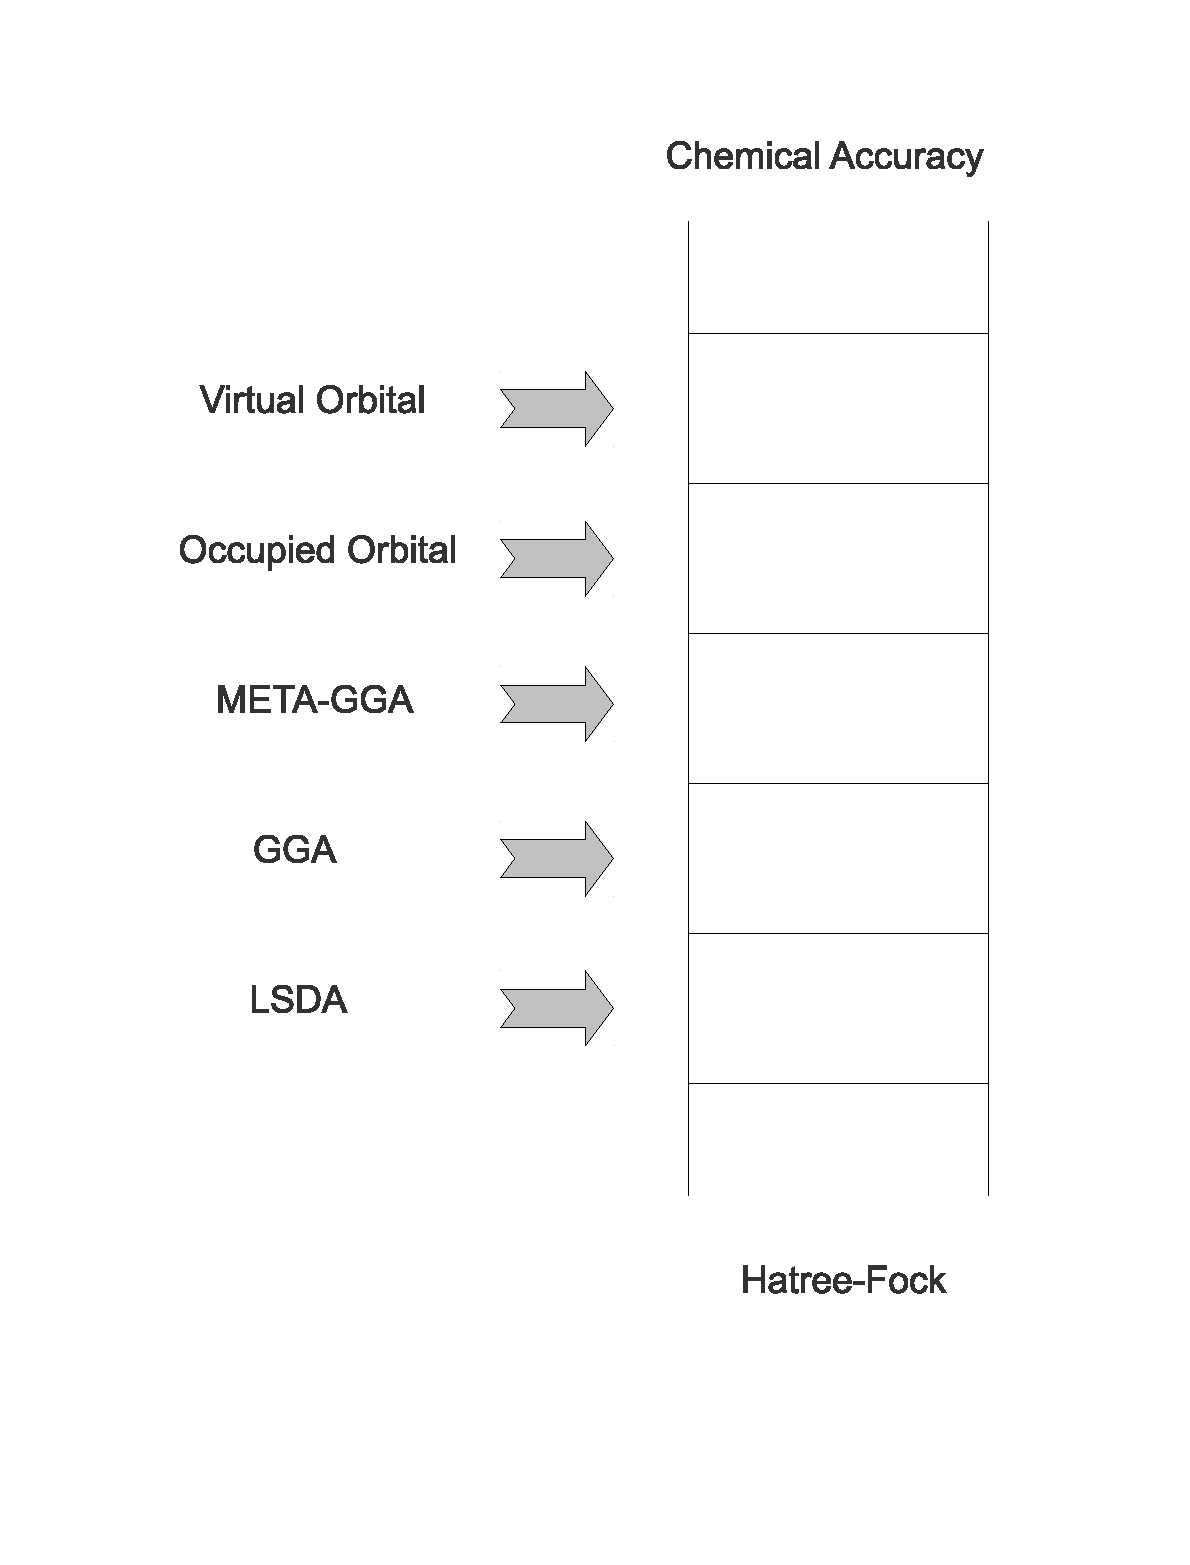
\includegraphics[scale=0.7]{jacob.eps}
\caption{Jacob's ladder for density functional approximation}
\end{center}
\end{figure}


%%%%%%%%%%%%%%%%%%%%%%%%%%%%%%%%%%%%%%%%%%%%%%%%%%%%%%%%%%%%%%%%%%%%%%%%%%%
\section{The Kohn-Sham equation}
\label{DFTI:4}
%
%
%
By this point, actually we have been set up all of the important
concepts for initialize the concrete calculation.

In the Kohn-Sham scheme, the approximated single electron wave
function for the non-interacting system is used to minimize the
total energy expression we have gotten in the (\ref{DFTIeq:24}).
Follows the tradition in the above section, here the $\theta_{i}$ is
employed to represent the Kohn-Sham orbital. And the $\phi$ is
always used to denote the atomic orbitals; so as to distinguish the
KS orbital. Furthermore, the condition for the Kohn-Sham orbitals is
just put forward in the (\ref{DFTIeq:27}) and (\ref{DFTIeq:28}).

Now the physical meaning of $\theta_{i}$ is clear. Since the
$\theta_{i}$ is the eigen states for single electron operator, then
we can use it to form some Slater determinant to represent the whole
quantum state:
\begin{equation}
\label{DFTIeq:11}
  \Theta_{KS}=\frac{1}{\sqrt{n!}}   \left | \begin{array}{cccc}
      \theta_{1}(1) & \theta_{2}(1) & \cdots & \theta_{n}(1) \\
      \theta_{1}(2) & \theta_{2}(2) & \cdots & \theta_{n}(2) \\
      \cdots & \cdots & \cdots & \cdots                      \\
      \theta_{1}(n) & \theta_{2}(n) & \cdots & \theta_{n}(n)
    \end{array} \right |
\end{equation}
Here we restrict ourself to the close shell case, hence the spin
state for the orbitals is not considered here. The $\Theta_{KS}$ has
the form: $|\Theta_{KS}|^{2}=\rho$.

So far the energy is expressed as:
\begin{equation}\label{}
  E[\rho]=T_{S}[\rho]+J[\rho]+E_{v}[\rho]+E_{XC}[\rho]
\end{equation}

With each term explicitly expressed in the energy expression, it
finally yields:
\begin{multline}\label{}
  E[\rho]=
  -\frac{1}{2}\sum_{i}^{n}\langle\theta_{i}(r)|\nabla^{2}|\theta_{i}(r)\rangle
  -\sum_{i}^{n}\sum_{A}^{N}\int\frac{Z_{A}}{r_{iA}}|\theta_{i}(r)|^{2}dr+ \\
  \frac{1}{2}\sum_{i}^{n}\sum_{j}^{n}
  \int\int|\theta_{i}(r)|^{2}\frac{1}{|r-r^{'}|}|\theta_{j}(r^{'})|^{2}drdr^{'}
  +E_{XC}[\rho(r)]
\end{multline}

Here we can strike up the variational search among the $\theta_{i}$,
just the same procedure which has been carefully described in the
chapter \ref{HFT}.

So the final KS equation is:
\begin{equation}\label{DFTIeq:12}
  \left [ -\frac{1}{2}\nabla^{2} + \hat{V}_{S}(r) \right ] \theta_{i}(r) =
  \epsilon _{i}\theta_{i}(r)
\end{equation}

The $\hat{V}_{S}(r)$ is:
\begin{equation}\label{DFTIeq:13}
  \hat{V}_{S} = v(r) + \sum_{i}^{n}\int\frac{|\theta_{i}(r^{'})|^{2}}
  {|r-r^{'}|}\,\,
  dr^{'}
  + \frac{\delta E_{XC}[\rho]}{\delta \rho(r)}
\end{equation}

Here let me note something more for the functional for the classic
electron repulsion:
\begin{align}\label{}
J[\rho] &=
\frac{1}{2}\int\int\frac{\rho(r)\rho(r^{'})}{|r-r^{'}|}drdr^{'}
\Rightarrow \nonumber \\
J[\rho] + J[\delta\rho] &= \frac{1}{2}\int\int\frac{(\rho(r) +
\delta\rho(r))(\rho(r^{'}) +
\delta\rho(r^{'}))}{|r-r^{'}|}drdr^{'} \Rightarrow \nonumber \\
J[\delta\rho] &= \frac{1}{2}\int\int\frac{\rho(r)
\delta\rho(r^{'})}{|r-r^{'}|}drdr^{'} +
\frac{1}{2}\int\int\frac{\delta\rho(r)\rho(r^{'})}{|r-r^{'}|}drdr^{'}
\nonumber \\
&=\int\int\frac{\rho(r)\delta\rho(r^{'})}{|r-r^{'}|}drdr^{'}
\end{align}
Theretofore, the factor of $1/2$ has been removed in the functional.
More discussion about the derivatives for the energy and functional
will be shown in the following content.


%%%%%%%%%%%%%%%%%%%%%%%%%%%%%%%%%%%%%%%%%%%%%%%%%%%%%%%%%%%%%%%%%%%%%%%%%%%%%
\section{Spin polarized Kohn-Sham function}
%
%
%
%
Now let's introduce spin polarized Kohn-Sham function, which is some
simple extension to the Kohn-Sham equation we have introduced.

In the density matrices section, we have known that the density
matrices actually depending on the spin variables on the location of
$r$ (see the section \ref{DODM_in_density_matrices}). Therefore, we
can also consider the up and down spin as separate variables, so to
define the spin density as:
\begin{equation}
\label{eq:FIDFTeq:76} \rho_{\sigma}(r) = n \int |\Psi(r, \sigma,
x_{2}, x_{3}, \cdots, x_{n})|^{2} dx_{2}dx_{3}\cdots dx_{n}
\end{equation}
While here the $\rho_{\sigma}(r)d^{3}r$ characterizes the density to
find an electron of spin $\sigma$ in $d^{3}r$ around the location of
$r$. Usually the spin density is characterized as $\rho^{\alpha}(r)$
and $\rho^{\beta}(r)$, or the $Q(r) = \rho^{\alpha}(r) -
\rho^{\beta}(r)$ plus the total density $\rho(r) = \rho^{\alpha}(r)
+ \rho^{\beta}(r)$.

So why we introduce the spin density into the Kohn-Sham equation?
Firstly, it's some necessary generalization for the system in
presence of an external magnetic field. For example, the electron
spin susceptibility, and the spin-orbit-coupling etc. They can be
only included within the spin density framework.

However, the major advantage for the spin polarized Kohn-Sham
function is that it leads to some more accurate system description.
For example, for the system with unpaired electrons, such as $Li$
atoms; the spin up density is unable to equal to the spin down type
density; so the close shell type of description is surely bad for
this situation.

Now let's go to see how to express the Kohn-Sham equation in the
spin density framework. Since the spin variable is introduced, the
Kohn-Sham orbital in the non-interacting system should also include
the spin variables; so that the Kohn-Sham orbitals should satisfy
the condition below (here we use $p$ to signal the $\alpha$
electron, and $q$ to designate the $\beta$ electrons):
\begin{align}
  \label{DFTIeq:77}
    \sum_{i=1}^{p}\theta^{2}_{i\alpha}(r) &=
    \rho^{\alpha}(r) \nonumber \\
    \sum_{i=1}^{q}\theta^{2}_{i\beta}(r) &=
    \rho^{\beta}(r)
\end{align}
While the non-interacting restriction requires that the
orthogonality condition that:
\begin{equation}
  \label{DFTIeq:78}
\int \theta^{*}_{i\sigma}(r)\theta_{j\sigma^{'}}(r) d\bm{r} =
\delta_{ij}\delta_{\sigma\sigma^{'}}
\end{equation}

Based on the (\ref{DFTIeq:77}) and (\ref{DFTIeq:78}), compared with
the (\ref{DFTIeq:11}) we can construct the spin dependent Slater
determinant as:
\begin{equation}
\label{DFTIeq:79} \Theta_{KS} =
 \begin{vmatrix}
         \theta_{1}(1)\alpha(1)  & \cdots  & \theta_{p}(1)\alpha(1)
       & \theta_{p+1}(1)\beta(1) & \cdots  & \theta_{n}(1)\beta(1)  \\
         \theta_{1}(2)\alpha(2)  & \cdots  & \theta_{p}(2)\alpha(2)
       & \theta_{p+1}(2)\beta(2) & \cdots  & \theta_{n}(2)\beta(2)  \\
          \cdots                 & \cdots  & \cdots
       &  \cdots                 & \cdots  & \cdots                  \\
         \theta_{1}(n)\alpha(n)  & \cdots  & \theta_{p}(n)\alpha(n)
       & \theta_{p+1}(n)\beta(n) & \cdots  & \theta_{n}(n)\beta(n)  \\
       \end{vmatrix}
\end{equation}
We can see that the (\ref{DFTIeq:79}) is similar to the UHF wave
function we get in the (\ref{HFTeq:45}). By the similar procedure,
we can also get the total energy expression:
\begin{multline}
  \label{DFTIeq:80}
  E[\rho^{\alpha}, \rho^{\beta}] =
\sum^{p+q}_{i\sigma} \left\langle\theta_{i\sigma}
\left|-\frac{1}{2}\nabla^{2}\right| \theta_{i\sigma}\right\rangle +
\frac{1}{2}\sum^{p+q}_{i\sigma}\sum^{p+q}_{j\sigma^{'}} \langle
\theta_{i\sigma}\theta_{j\sigma^{'}}|\frac{1}{r -
  r^{'}}|
\theta_{i\sigma}\theta_{j\sigma^{'}} \rangle \\
+ \int v(r)\rho^{\alpha}(r)d^{3}r + \int v(r)\rho^{\beta}(r)d^{3}r +
E_{XC}[\rho^{\alpha}, \rho^{\beta}]
\end{multline}

Here we can see that the kinetic part and the classic coulomb part
are independent to the spin variables.

Then, the variational research is carried out under the
orthogonality restriction in the (\ref{DFTIeq:78}), similar to the
treatment in the part of (\ref{RHFUHF_in_HF}), we can get a pair of
functions:
\begin{align}
\label{DFTIeq:81} \left[-\frac{1}{2}\nabla^{2} +
  V_{\alpha}(r)\right]\theta_{i\alpha}(r) &=
\epsilon_{i\alpha}\theta_{i\alpha}(r) \nonumber \\
\left[-\frac{1}{2}\nabla^{2} +
  V_{\beta}(r)\right]\theta_{i\beta}(r) &=
\epsilon_{i\beta}\theta_{i\beta}(r)
\end{align}

Where the spin dependent effective potentials are:
\begin{align}
  \label{DFTIeq:82}
V_{\alpha}(r) &= v(r) + \int\frac{\rho(r^{'})}{r -
  r^{'}}dr^{'} +
\frac{\delta E_{XC}[\rho^{\alpha}, \rho^{\beta}]}{\delta
  \rho^{\alpha}(r)} \nonumber \\
V_{\beta}(r) &= v(r) + \int\frac{\rho(r^{'})}{r -
  r^{'}}dr^{'} +
\frac{\delta E_{XC}[\rho^{\alpha}, \rho^{\beta}]}{\delta
  \rho^{\beta}(r)}
\end{align}

Now we can see that the results is very similar to the UHF
framework, however; they retains very different physical meanings.



%%%%%%%%%%%%%%%%%%%%%%%%%%%%%%%%%%%%%%%%%%%%%%%%%%%%%%%%%%%%%%%%%%%%%%%%%%%%%
\section{Further discussion for the $T_{S}[\rho]$}
\label{DFTI:3}
%
%  what's the relation between the Ts[\rho] and T[\rho]?
%  another understanding about the $T_{S}[\rho]$
%
Through the Kohn-Sham equation in (\ref{DFTIeq:12}), we can get the
KS orbital of $\theta_{i}(r)$ to minimize the whole energy so that to
get the expression of $T_{S}[\rho]$. However, as in the derivation of total
energy expression, we have a question that how to understand the physical
meaning of $T_{s}[\rho]$? Here we will have an answer.

Firstly we can define the $T_{S}[\rho]$ in some constrained search way:
\begin{equation}\label{}
\begin{split}
T_{S}[\rho] &= \min_{\Psi_{D} \rightarrow \rho}
\langle\Psi_{D}|\hat{T}|\Psi_{D}\rangle \\
    &= \min_{\sum_{i=1}^{n}|\psi_{i}|^{2} \rightarrow \rho}
    \left[\sum_{i=1}^{n}\int\psi^{*}_{i}(r)
    \left(-\frac{1}{2}\nabla^{2}\right)\psi_{i}(r)dr\right]
\end{split}
\end{equation}
Here the $\Psi_{D}$ indicates the anti-symmetric $n$ non-interacting 
electron wave functions, and it's composed by some $n$ non-interacting
orbitals of $\psi_{i}$. The constraint search is over all the $\Psi_{D}$ 
which gives the real density of $\rho$.

Interestingly we can prove that such definition can also lead to the
Kohn-Sham equation in (\ref{DFTIeq:12}). Firstly let's define some
functional:
\begin{multline}\label{}
\Omega(\psi_{1}, \psi_{2}, \cdots, \psi_{n}) =
\sum_{i=1}^{n}\int\psi^{*}_{i}(r)
    \left(-\frac{1}{2}\nabla^{2}\right)\psi_{i}(r)dr \\
    +
\int\lambda(r)\left\{\sum_{i=1}^{n}|\psi_{i}(r)|^{2}
-\rho(r)\right\}dr -
\sum_{ij}^{n}\epsilon_{ij}\int\psi^{*}_{i}(r)\psi_{j}(r)dr
\end{multline}
Here inside the $\Omega$ we have introduced the Lagrangian
multiplier of $\lambda(r)$ and $\epsilon_{ij}$. $\lambda(r)$ is used
to make sure that the density between the non-interacting system and
the real system is same, and $\epsilon_{ij}$ is used to require the
orthogonality between the non-interacting of $\psi_{i}(r)$.

The energy minimization condition is given by:
\begin{equation}\label{}
\frac{\partial \Omega}{\partial \psi_{k}} = 0 \quad k=1, 2, \cdots,
n
\end{equation}
Then we can get the resulting equation:
\begin{equation}\label{DFTIeq:16}
\begin{split}
  \hat{h}_{s}\psi_{k}(r) &= \sum_{l=1}^{n}\epsilon_{kl}\psi_{l}(r) \\
    \hat{h}_{s} &=-\frac{1}{2}\nabla^{2} + \lambda(r)
\end{split}
\end{equation}
Hence, the $\lambda(r)$ can be viewed as some local potential which
is just corresponding to the $\hat{V}_{s}(r)$ in (\ref{DFTIeq:13}),
and the $\psi_{k}(r)$ is just corresponding to the $\theta_{i}(r)$
in (\ref{DFTIeq:12}). On the other hand, such derivation is giving
the same Kohn-Sham equation again! Hence we can say, the physical 
meaning of non-interacting orbitals in Kohn-Sham framework is to 
minimize the $T_{s}[\rho]$.

Now let's proceed to another question that how close between the
$T_{S}[\rho]$ and the real kinetic energy in DFT?

Before answering the question, we should make it clear that how to
express the real kinetic energy in DFT. According to Levy constraint
search in (\ref{DFTI:1}), the kinetic energy as well as the
repulsion energy in DFT can given by the functional of
$F_{HK}[\rho]$:
\begin{equation}\label{}
F_{HK}[\rho] = \min_{\psi\rightarrow\rho}
\langle\psi|T+V_{ee}|\psi\rangle
\end{equation}
Where the $\psi$ indicates all the wave functions which give the
density of $\rho$. If we label the kinetic energy in the
$F_{HK}[\rho]$ as $T[\rho]$, then simply we can have:
\begin{equation}\label{DFTIeq:14}
T_{S}[\rho] \leq T[\rho]
\end{equation}
Since the wave function of $\psi$ in the $F_{HK}[\rho]$ may not
corresponding to the wave function which is just minimizing the
kinetic energy. Here the proof is just paraphrastic, the more strict
proof should refer to the material given by Weitao\cite{weitaoYang}.

The inequation in (\ref{DFTIeq:14}) has some significant consequence
that the exchange correlation functional contains some positive
component of kinetic energy. In the discussion related to the
functional, we will analyze it again.

%%%%%%%%%%%%%%%%%%%%%%%%%%%%%%%%%%%%%%%%%%%%%%%%%%%%%%%%%%%%%%%%%%%%%%
\section{How to code the exchange-correlation energy}
\label{sec:XC_functional}
%
%
%
%
Now in this section, we are going to give a discussion that how to
code the conceptual XC functional so that we can calculate the energy,
first and second derivatives etc. within DFT framework. For
simplicity, let's restricted the discussion within the ground state
DFT calculation first.

In the ground state DFT calculation, compared with the traditional
wave function method; there are two things we needed to get the
information of the system we study:
\begin{align}
 \label{eq:XC_functional.1}
\text{wave function} &\Leftrightarrow \text{electron density}
\nonumber
\\
\text{operator on the wave function} &\Leftrightarrow \text{functional
  on the density}
\end{align}
The density here we are talking about, is the electron density from
the non-interacting system which is in one to one mapping relationship
with the real system. Through the imaginary Kohn-Sham orbitals (see
\ref{DFTI:2} for more information), we can construct the electron
density for the real system.

On the other hand, how can we derive the electron density? We have
Kohn-sham equation, which is similar with Hatree-Fock equation (more
details about the KS equation please see \ref{DFTI:4}), through that
equation the trial density firstly generated by guess will be renewed,
then the newer electron density will be brought into the whole
function again until the self-consistent condition is met. Finally, by
the result electron density we can evaluate all the system information
we need.

In the Kohn-Sham equation in (\ref{DFTIeq:12}), we have an item which
contains the exchange and correlation energy, its general form has
been detailed discussed in the chapter \ref{Functionals_in_DFT}. In
that chapter, we derived the general relation between energy and the
density, the gradient of density or even the Laplacian of density
(in meta-GGA form) from the fundamental physical laws, and finally
their explicit forms are finally gotten. If both of the explicit form
of XC functional and the trial density is known, we can get the result
density through KS equation.

Finally, there's a question left that how to construct the trial
density, or more properly to say, the trial Kohn-Sham orbitals? In
principle, we can find enormous ways to do this, but in practice we
construct the trial density from the traditional AO basis set
functions, in other words;  the GTO or STO functions:
\begin{align}
  \label{eq:XC_functional.2}
\phi_{i} &= \sum_{j}d_{ij}\chi_{j} \Rightarrow \nonumber \\
\varphi_{i} &= \sum_{j}^{n}c_{ij}\phi_{i} \Rightarrow \nonumber \\
\rho_{trial} &= \sum_{i}^{occ}\varphi_{i}^{*}\varphi_{j} \nonumber \\
&=
\sum_{i}^{occ}\sum_{j}^{n}\sum_{k}^{n}c_{ij}^{*}c_{ik}\phi_{j}^{*}
\phi_{k}
\nonumber \\
&= \sum_{j}^{n}\sum_{k}^{n}P_{jk}\phi_{j}^{*}\phi_{k}
\end{align}
Here, the $\chi$ is the basic functions to form the basis set
functions
$\phi$, the $\chi$ can be GTO or STO; but mostly we use GTO. Here in
this step, the basis set functions are same between the wave function
method and the new DFT method. Then based on the basis set functions
of $\phi$, we can construct the trial Kohn-Sham orbitals of $\varphi$,
so finally we can get the trial density. Here above the $P_{jk}$ is
the density matrix for the basis function of $\phi_{j}$ and
$\phi_{k}$. 

Here we have something important to mention. In real culculation, we
always use basis sets in quantum chemistry, that is to say; all the
function space are built from some ``delicately selected'' basis
functions:
\begin{align}
 \label{basis_idea_funtional_eq:1}
\text{GTO (STO)} &\longrightarrow \text{AO  (basis sets)} \nonumber \\
\text{AO} &\longrightarrow \text{MO} \nonumber \\
\text{MO} &\longrightarrow \text{Slater determinants}
\end{align}
Here in such process, the basic function (GTO or STO) are fixed, the
forming of function space are all depending on their coefficients.
Specifically, in the (\ref{eq:XC_functional.2}) each basis sets of
$\phi_{i}$ is fixed, the coefficient of $d_{ij}$ and $\chi_{j}$ (GTO
or STO) are all pre-determined. On the other hand, $c_{ij}$ are
varied according to the energy variation process (could be HF method
or Kohn-Sham method), so the $\varphi_{i}$ (MO) are just some
variation results based on the space expanding by the $c_{ij}$. So
here we can see that $c_{ij}$ is the only thing varied, and we are
seeking for in energy calculation. 

In practice, the coefficient of the $c_{ij}$ is in $n\times n$
dimension ($n$ basis sets forming $n$ MOs). On the other hand, we can
also use the density matrix of $P_{ij}$ to equivalently express the
space of $c_{ij}$ (it's also in $n\times n$ dimension). Hence the
enegy variation process can be viewed as:
\begin{equation}
 \label{basis_idea_funtional_eq:2}
E = \Psi (q, P_{ij}, \cdots)
\end{equation}  
This is the central idea we applied across the quantum software.

Finally, let's come back to the solving of KS equation. if we
compare the HF equation and the KS equation, we can
find out that the only difference btween them is that there's a new
item of $E_{XC}$ in KS equation (here the point is aiming at the
hybrid functionals because it contains the HF exchange part, for
pure functional method such as BLYP; there's no HF exchange part),
and all the other terms are kept to be same. Hence let's proceed to
discuss the formation of $E_{XC}$ in details.

%%%%%%%%%%%%%%%%%%%%%%%%%%%%%%%%%%%%%%%%%%%%%%%%%%%%%%%%%%%%%%%%%%%%%%


%%% Local Variables:
%%% mode: latex
%%% TeX-master: "../../main"
%%% End:
